\section{Experimental Methods}

\subsection{\label{sec:setup} Experimental setup}

\begin{figure}[h]
    \centering
    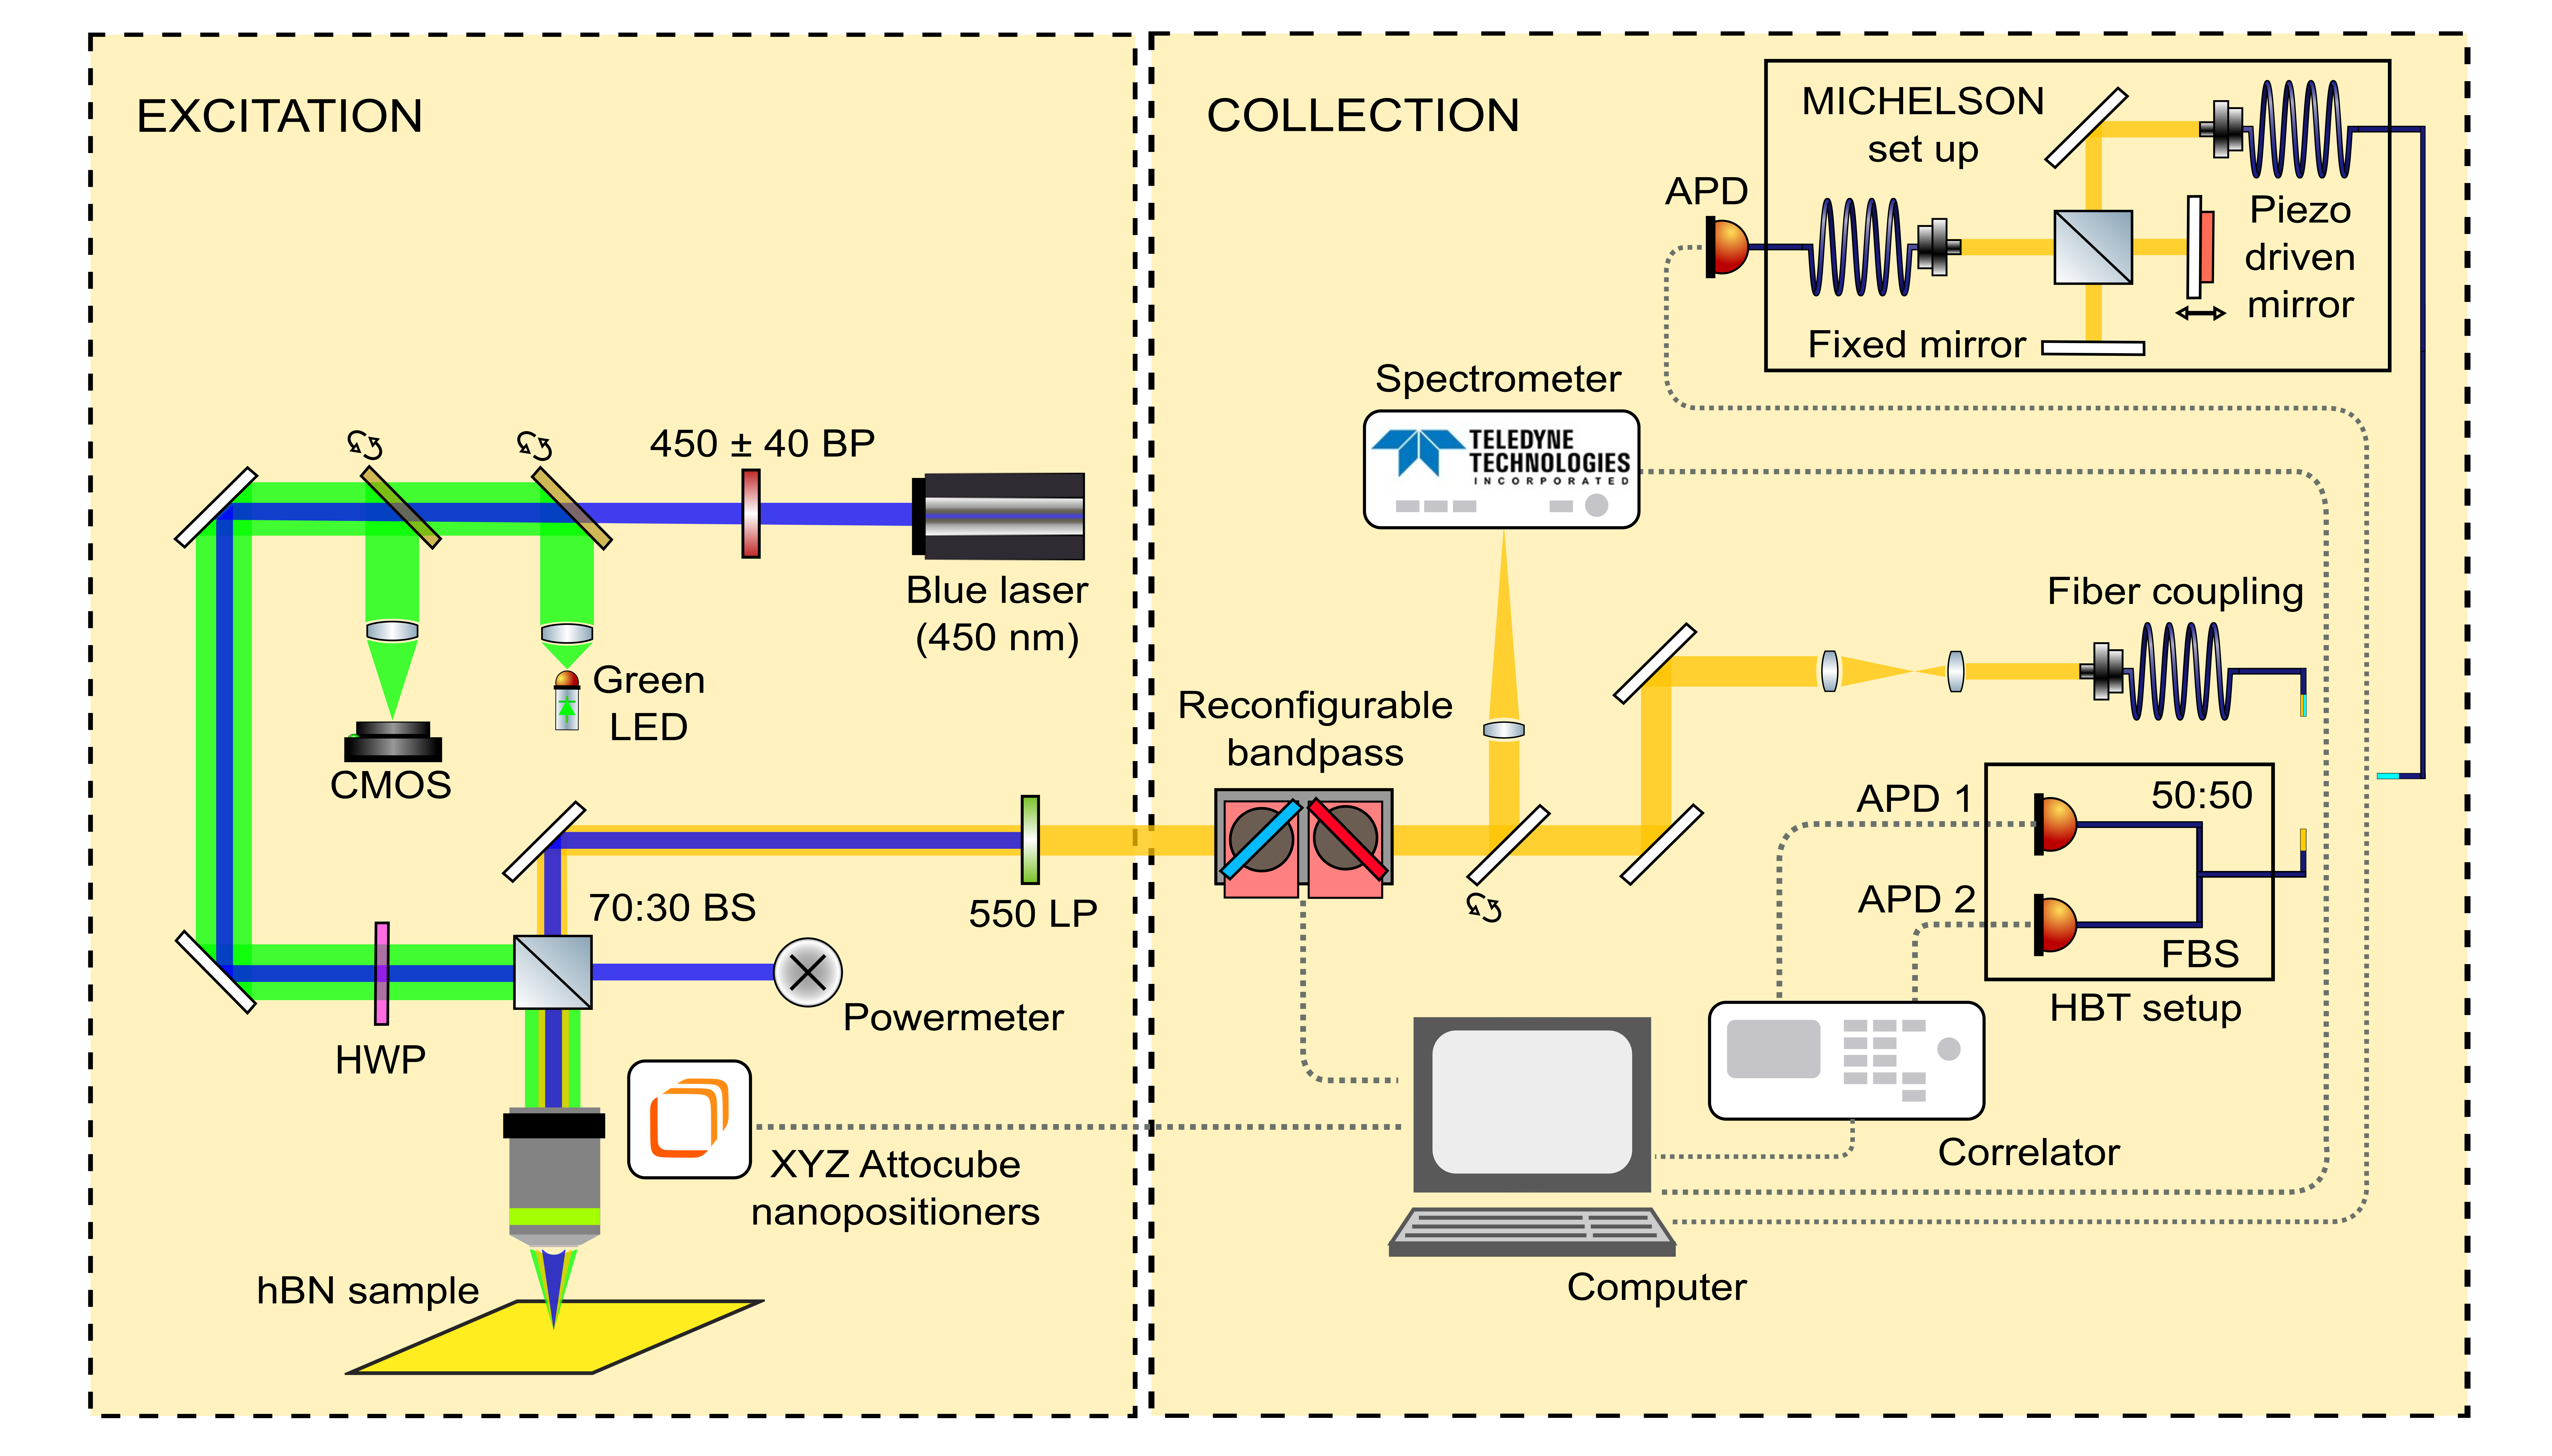
\includegraphics[width=1\linewidth]{Figures/ExperimentalSetUp.png}
    \caption{Schematic of the confocal microscopy setup used for the non-resonant excitation and collection of photoluminescence from defect centres in hexagonal boron nitride (hBN). Excitation is provided by a 450~nm blue laser, spectrally filtered and polarisation-controlled via a bandpass filter and a half-wave plate (HWP), respectively. A 70:30 beam splitter directs the beam to the sample while allowing photoluminescence to pass into the collection path. Sample imaging and alignment are achieved using a 532~nm green LED and a CMOS camera, with the sample mounted on a closed-loop XYZ Attocube nanopositioning stage. Emission is initially filtered by a 550~nm long-pass filter and further spectrally selected using a tunable reconfigurable bandpass filter (Semrock, 615--710~nm, 2~nm FWHM minimum). The filtered signal is then directed either to a spectrometer for spectral analysis or fibre-coupled for photon statistics and coherence measurements. Fibre-coupled photons can be sent to a Hanbury Brown and Twiss (HBT) setup for $g^{(2)}(0)$ measurements or a free-space Michelson interferometer to assess photon coherence. Avalanche photodiodes (APDs) are used for detection, and all time-resolved data is processed via a time-correlated single-photon counting (TCSPC) module.}
    \label{fig:setup}
\end{figure}

A confocal microscopy setup was used at room temperature for the non-resonant excitation and collection of photoluminescence from defect centres in hexagonal boron nitride (hBN), as shown in Fig.~\ref{fig:setup}. A 532~nm green LED and a CMOS camera were used to illuminate and image the sample surface, enabling visual identification and alignment of potential defect sites. Initially, a red LED (\textcolor{red}{XXX~nm}) was used to match the excitation position more closely to the single-photon emission wavelength, ensuring optimal alignment. However, this wavelength lies within the stopband of the cavity mirrors, making the sample invisible when viewed through the top concave mirror. In contrast, the 532~nm green LED lies outside the stopband, allowing the sample to be visualised even with the cavity in place. Although the focal lengths for the red and green illumination differ slightly, the discrepancy was found to be minimal for practical alignment. The sample was mounted on a set of closed-loop XYZ Attocube nanopositioners, which allow for precise positioning in all three spatial dimensions.


Excitation was performed using a 450~nm blue PicoQuant laser, spectrally cleaned with a 450~$\pm$~40~nm bandpass filter. A half-wave plate (HWP) was inserted into the excitation path to control the laser polarisation, allowing optimisation of the excitation conditions. A 70:30 (transmission:reflection) beam splitter was used to direct the excitation light towards the sample while transmitting the collected emission into the collection path. The actual ratio of the beam splitter transmissoin and reflection at the excitation wavelength was measured to be 83:17. Although a dichroic mirror would theoretically offer higher collection efficiency, its use was impractical in this setup. Throughout the project, both the excitation and illumination wavelengths were frequently changed, requiring different dichroics to be swapped in and out. The additional complexity and alignment overhead outweighed the potential gains in efficiency. The beam was focused onto the sample using a \textcolor{red}{Mitutoyo} objective lens with a numerical aperture of 0.55, mounted on a New Focus micropositioner for precise Z-axis control.


Photoluminescence from the sample was filtered by a 550~nm long-pass filter to reject scattered excitation light. Further spectral filtering was achieved using a pair of motorised, tunable Semrock filters (704~nm short-pass and long-pass), configured as a reconfigurable bandpass filter tunable between 615--710~nm with a minimum FWHM of 2~nm. The filtered emission can be directed either to a spectrometer for spectral analysis or coupled into a single-mode optical fibre.

The fibre-coupled light can be routed to a Hanbury Brown and Twiss (HBT) setup for photon correlation measurements or to a free-space Michelson interferometer for temporal coherence characterisation. The HBT setup uses a 50:50 fibre beam splitter to direct the signal to two avalanche photodiodes (APDs), with the arrival times recorded by a QuTag time-correlated single-photon counting (TCSPC) module. The Michelson interferometer consists of a 50:50 beam splitter with one arm terminating in a fixed mirror and the other in a mirror mounted on a piezoelectric actuator. This piezo was integrated into a motorised translation stage, enabling both coarse (millimetre scale) and fine (nanometre scale) path length adjustment. One of the output arms was coupled into a single-mode fibre and detected by an APD.

\subsubsection{Detection Scheme}

A \textcolor{red}{Teledyne Technologies spectrometer} with a \textcolor{red}{princeton instruments CCD} was uses for spectral characterisation of the emitters. The spectrometer had grating options of 150 gratings per millimeter (g/mm), 300 g/mm and 600 g/mm. The majority of the time the 300 g/mm grating was used as it provided a good balance between spectral resolution and range. This combination of slit and CCD provided a spectral range of $86.1$ nm and a resolution of \textcolor{red}{Use Mercury lamp or mattise laser and measure FWHM.} nm. The data from the spectrometer was then visualised in the Lightfield application.



Six fibre-coupled avalanche photodiodes (APDs) were available in the laboratory, comprising two different detector types. These detector provides a timing resolution of 35~ps (FWHM), a detection efficiency of approximately 28\% at 670~nm, an active area diameter of \textcolor{red}{X~$\mu$m}, a dark count rate of \textcolor{red}{X~Hz}, and a dead time of 77~ns. For experiments prioritising photon collection efficiency, such as second-order correlation measurements, \textcolor{red}{Thorlabs SPDMH2F} detectors were used. They offers a typical timing resolution of 1~ns, a quantum efficiency of around 70\% at 670~nm, a 100~$\mu$m active area diameter, a maximum dark count rate of 100~Hz, and a dead time of 45~ns.

To fully characterise the timing performance of each APD, their instrument response functions (IRFs) were measured. The IRF of an APD describes the temporal spread in the detector’s response to an ideally instantaneous photon arrival, and defines the effective timing resolution of the system. This characterisation was carried out using a pulsed \textcolor{red}{Tsunami laser} operating at a wavelength of 750~nm with a pulse width of approximately 3~ps, much shorter than the expected temporal resolution of the APDs. Each laser pulse was split using a 50:50 beam splitter: one path was directed to a fast photodiode to provide a reference trigger, while the other passed through a fibre attenuator before reaching the APD under test.

The trigger voltage levels for the APDs and the photodiode were selected such that the threshold corresponded to the point of maximum gradient of the respective electrical signal. For reference, the photodiode trigger signal was set to \textcolor{red}{-116~mV}. Table~\ref{tab:apd_characterisatoin} summarises the trigger voltages and signal durations for each APD tested in the laboratory.


\begin{table}[h!]
\centering
\begin{tabular}{|c|c|c|}
\hline
\textbf{APD Label} & \textbf{Trigger voltage (V)} & \textbf{Signal Length (ns)} \\
\hline
ThorLabs APD1 &     1.5        &      20        \\
\hline
Thorlabs APD2 &      1.2       &       20       \\
\hline
Thorlabs APD3 &      1.4       &       20       \\
\hline
Thorlabs APD4 &      1.3       &         20     \\
\hline
MPD APD1 &     1.5        &      23        \\
\hline
MPD APD2 &     1.5        &        23      \\
\hline
\end{tabular}
\caption{Trigger voltage and signal length for each APD}
\label{tab:apd_characterisatoin}
\end{table}

With the trigger level correctly set for each APD, first-order correlation data was collected between the reference signal from the photodiode and the subsequent detection signal from each APD, with a bin width of 1 ps. The results for Thorlabs APD1 and MPD APD1 are shown in Fig.~\ref{fig:apd-characterisation}. The FWHM of each APDs IRF was estimated in python by smoothing the raw data using the \texttt{savgol\_filter} function from the \texttt{scipy} library and measuring the FWHM of the smoothed curve. The APDs with the narrowest IRFs were selected for subsequent experiments to minimise timing uncertainty. MPD APD1 was used for lifetime measurements, while Thorlabs APD1 and APD3 were used for all other measurements.


\begin{figure}[h]
    \centering
    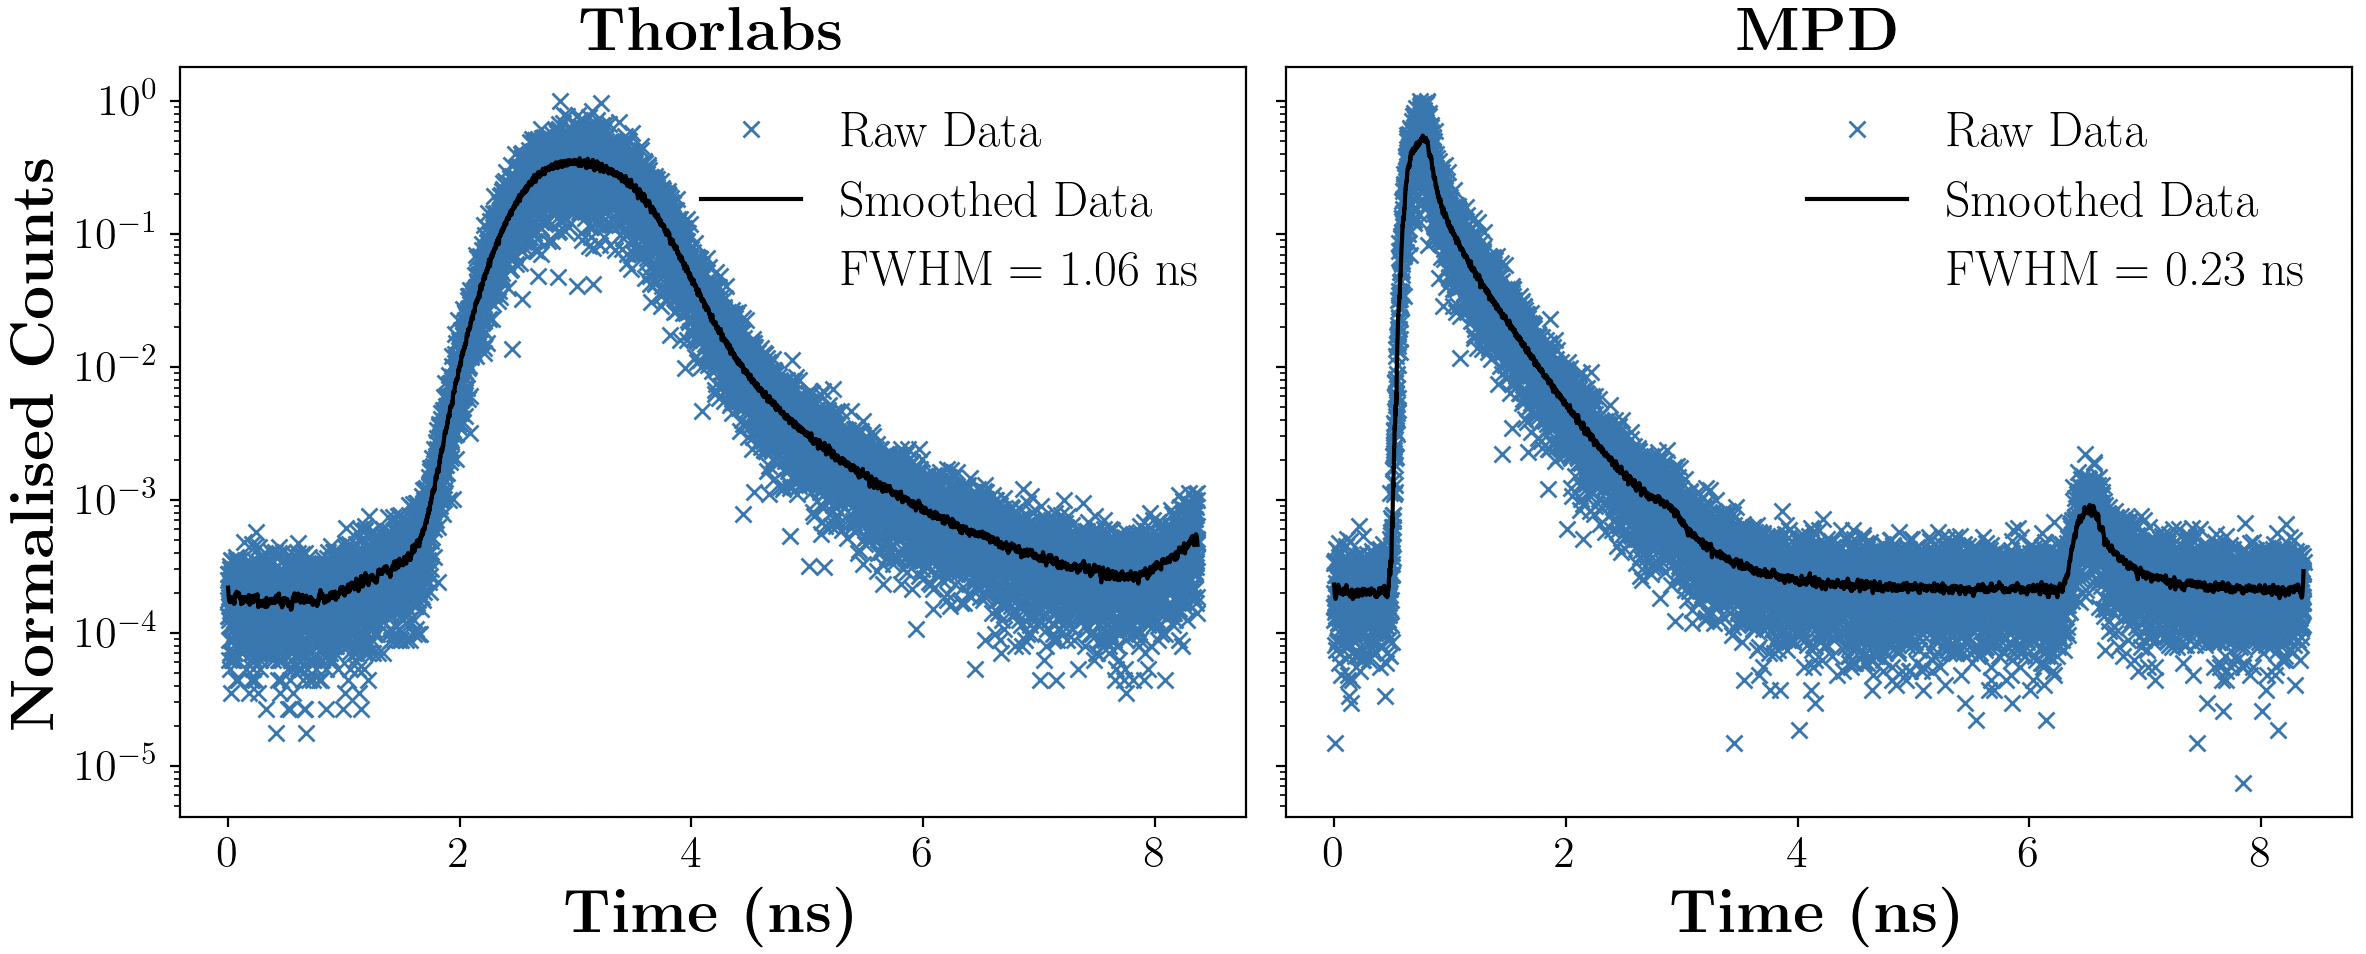
\includegraphics[width=0.9\linewidth]{Figures/APDChar.png}
    \caption{Instrument response functions (IRFs) of two representative avalanche photodiodes (APDs) measured using a 750~nm, $\sim$3~ps pulsed laser source. Raw data (green crosses) were smoothed using a Savitzky–Golay filter to extract the full width at half maximum (FWHM) of the IRF (black line). The Thorlabs detector exhibits an IRF of 1.06~ns FWHM, while the MPD detector demonstrates significantly sharper timing with a 0.23~ns FWHM.}
    \label{fig:apd-characterisation}
\end{figure}

The IRFs of both APDs, shown in Fig.~\ref{fig:apd-characterisation}, reflect the inherent differences in their timing performance. The Thorlabs APD displays a broader, more symmetric IRF consistent with a Gaussian profile, indicating greater timing jitter and a slower response. In contrast, the MPD APD exhibits a much sharper, asymmetric IRF with a rapid rise and an extended tail, characteristic of fast triggering and high temporal resolution, but with potential contributions from afterpulsing or delayed carrier effects. The secondary peak observed at approximately 6.5~ns in the MPD APD trace, as well as the rising signal at the end of the Thorlabs APD trace, can be attributed to signal reflections at BNC junctions within the detection circuitry.


\subsubsection{Laser Characterisation}

The laser employed was the PicoQuant LDH-IB-450-B laser head, controlled via a Taiko PDL M1 controller. It can operate in both CW and pulsed modes, and has a centre wavelength of 459~nm, as shown in Fig.~\ref{fig:laser-char}.

\begin{figure}[h]
    \centering
    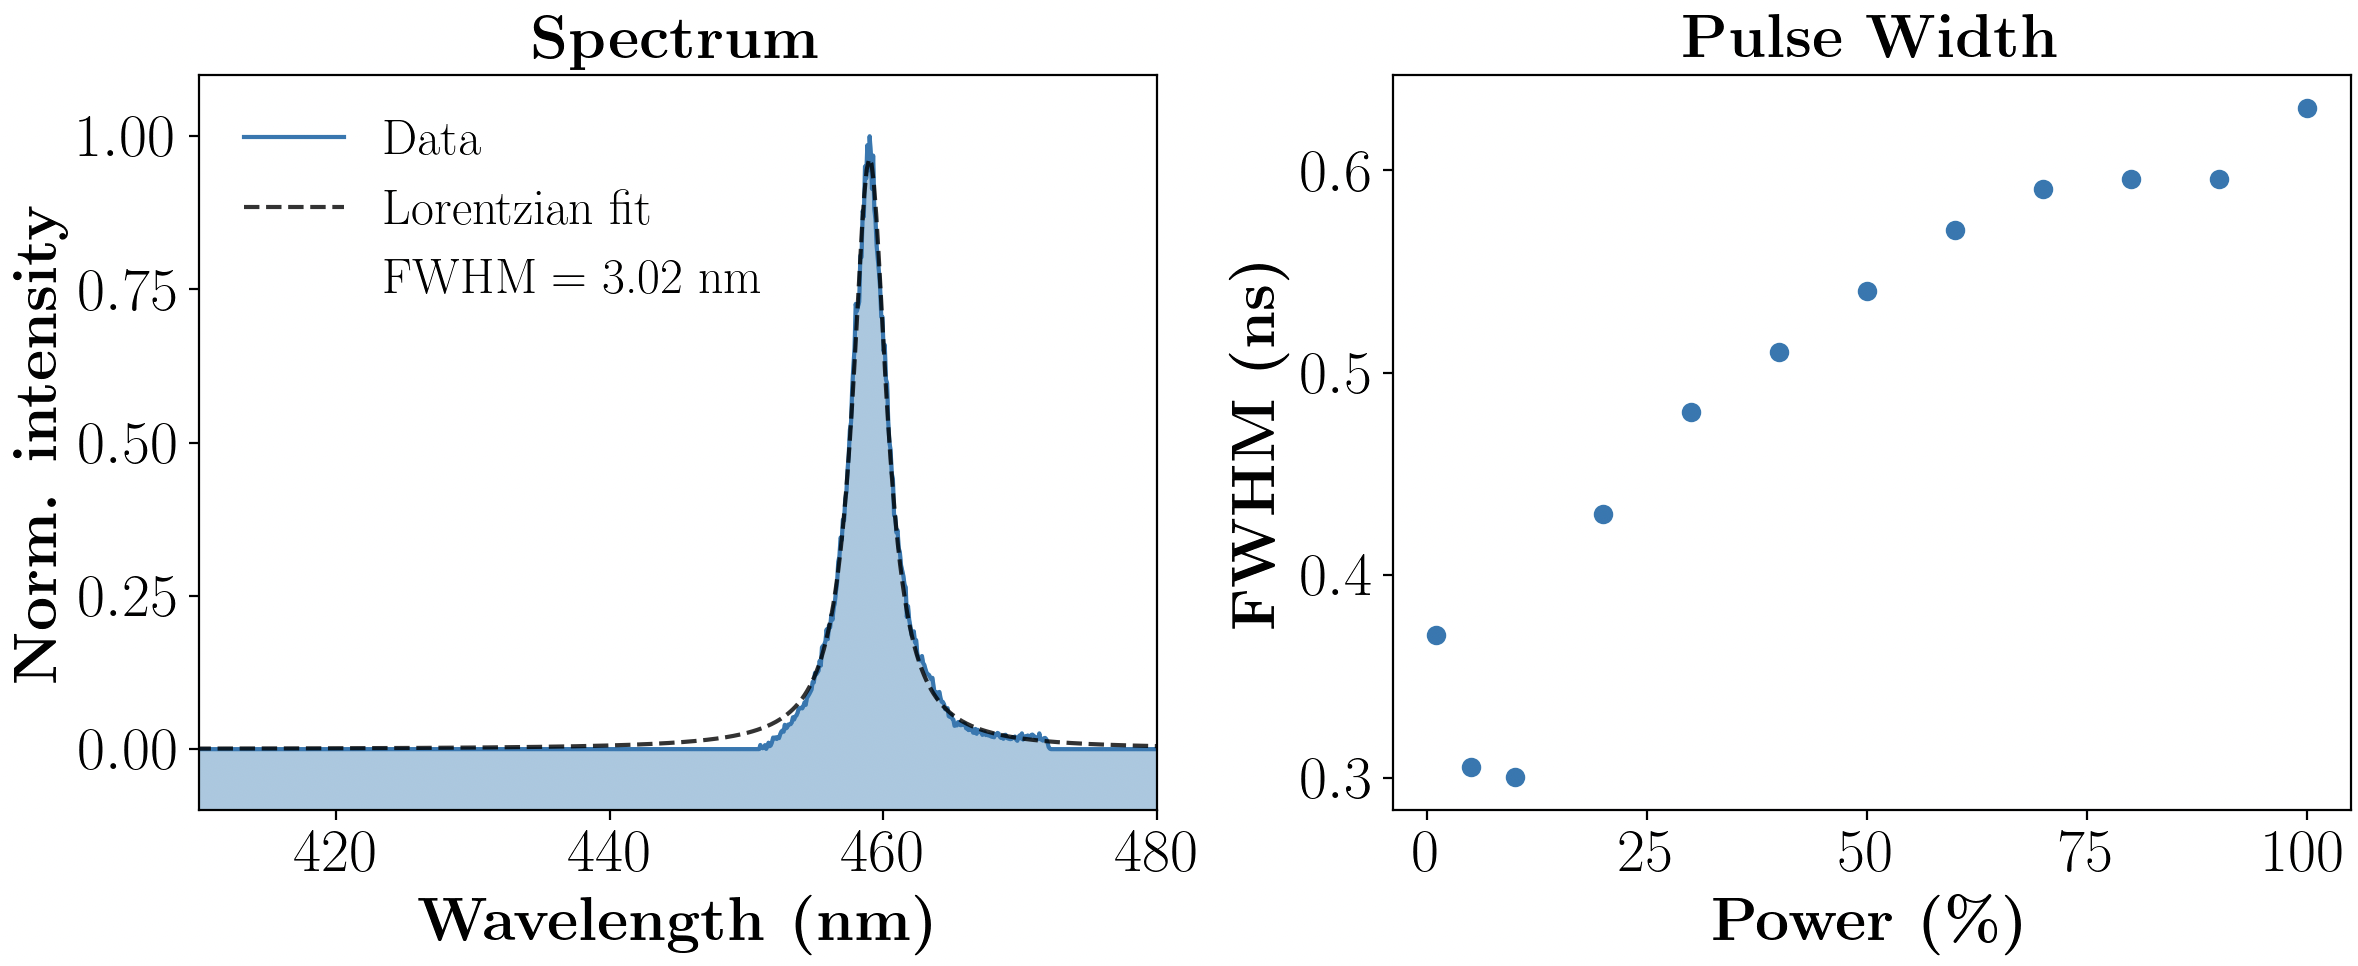
\includegraphics[width=0.9\linewidth]{Figures/LaserCharacterisation.png}
    \caption{Characterisation of the PicoQuant LDH-IB-450-B laser. (Left) Emission spectrum fitted with a Lorentzian function to extract the centre wavelength and FWHM, which was found to be 3.02~nm. (Right) Measured pulse width (FWHM) as a function of excitation power. A minimum pulse width is observed near 10\% laser power.}
    \label{fig:laser-char}
\end{figure}

The emission spectrum was recorded using a \textcolor{red}{Teledyne Technologies} spectrometer with the $450 \pm 40$~nm bandpass filter in place. The resulting spectrum was fitted with a Lorentzian function, yielding a full width at half maximum (FWHM) of 3.02~nm. The use of the bandpass filter was essential to suppress background noise, particularly in the 550--650~nm range, and to ensure a clean spectrum across the entire wavelength range of interest.

The pulse width of the emission was measured as a function of laser power using MPD APD1, figure \ref{fig:laser-char}. Since the measured FWHM values are close to the timing resolution of the detector itself, they should ideally be deconvoluted from the IRF. However, the absolute value of the pulse width is not of important in this context. What is more important is that it is minimised, which occurs around 10\% excitation power.

Although the laser used in this experiment operates in free space, an attempt was made to couple it into a single-mode fibre using a fibre collimator. However, the output beam from the laser head was highly elliptical, and even with the aid of cylindrical lenses to compensate for the asymmetry, a maximum coupling efficiency of only $\sim$30\% was achieved. Despite this limitation, coupling beams into single-mode fibres is generally desired, as it filters the spatial mode of the input beam, ensuring a well-defined Gaussian profile. To explore this further and aid in future setups, a program was developed to optimise the coupling efficiency of a free-space beam into a single-mode fibre.

Maximising single-mode coupling efficiency requires precise mode-matching between the spatial profile of the free-space laser beam and the output mode of the fibre collimator. In other words, the beam emerging from the laser must be transformed such that, at the input of the fibre collimator, it closely matches the divergence and waist of the beam that would emerge from the collimator itself. This condition can be experimentally verified by measuring the beam radius $w(z)$ as a function of propagation distance $z$ both directly from the laser head and from the backwards-emitted collimated beam. The two beam profiles should overlap in both width and curvature. Achieving this optimal transformation typically involves the use of a telescope composed of two carefully positioned lenses.

To automate this process, a Python program was developed to determine the lens configuration and spacing that best replicates the fibre-collimated beam profile. The program is based on Gaussian beam optics, where the beam radius as a function of propagation distance $z$ is described by:

\begin{equation}
    w(z) = w_0 \sqrt{1 + \left( \frac{z}{z_R} \right)^2},
    \label{eqn:beam-radius}
\end{equation}

where $w_0$ is the beam waist, and $z_R = \pi w_0^2 n / \lambda$ is the Rayleigh range, with $\lambda$ being the wavelength of the light and $n$ the refractive index of the medium. The beam radius $w(z)$ is defined as the radial distance at which the intensity drops to $1/e^2$ of its peak value.

The propagation of the Gaussian beam through optical elements is described using ABCD matrix formalism. For free-space propagation over a distance $x$, and transmission through a thin lens of focal length $f$, the respective matrices are:

\begin{equation}
    T_{fs} =
    \begin{pmatrix}
        1 & x \\
        0 & 1 
    \end{pmatrix}, \quad
    T_{l} =
    \begin{pmatrix}
        1 & 0 \\
        -\frac{1}{f} & 1 
    \end{pmatrix}.
    \label{eqn:beam-tm}
\end{equation}

By multiplying the appropriate sequence of matrices, the evolution of the beam through a two-lens system can be computed, allowing the predicted beam profile at the fibre input to be evaluated.

The program first fits the measured beam profiles from both the laser and fibre collimator to equation~\ref{eqn:beam-radius}, extracting the beam waist $w_0$ and Rayleigh range $z_R$ for each. It then performs a numerical optimisation to minimise the mean squared error (MSE) between the calculated beam profile (after passing through the two-lens system) and the experimentally measured fibre-collimated beam profile. This optimisation is implemented using \texttt{scipy.optimize.minimize}, subject to the following constraints: (1) a minimum allowable distance between the laser head and the first lens, accounting for any fixed optical elements in the path, and (2) the known distance between the laser and the fibre collimator. To ensure a global minimum is found, the optimisation is repeated 100 times with randomly initialised parameters, and the configuration yielding the lowest MSE is retained.

The script evaluates this optimisation across all valid combinations of lenses provided as input, with focal lengths specified by the user. The final output is the lens pair and corresponding positions that yield the closest match to the target fibre-collimated beam profile, thereby maximising the expected coupling efficiency. An example result of the optimisation process is shown in Fig.~\ref{fig:optimised-telescope}. The coupled light has an error of \textcolor{red}{XXX in $z_R$ and XXX in $\omega_0$}

\begin{figure}[h]
    \centering
    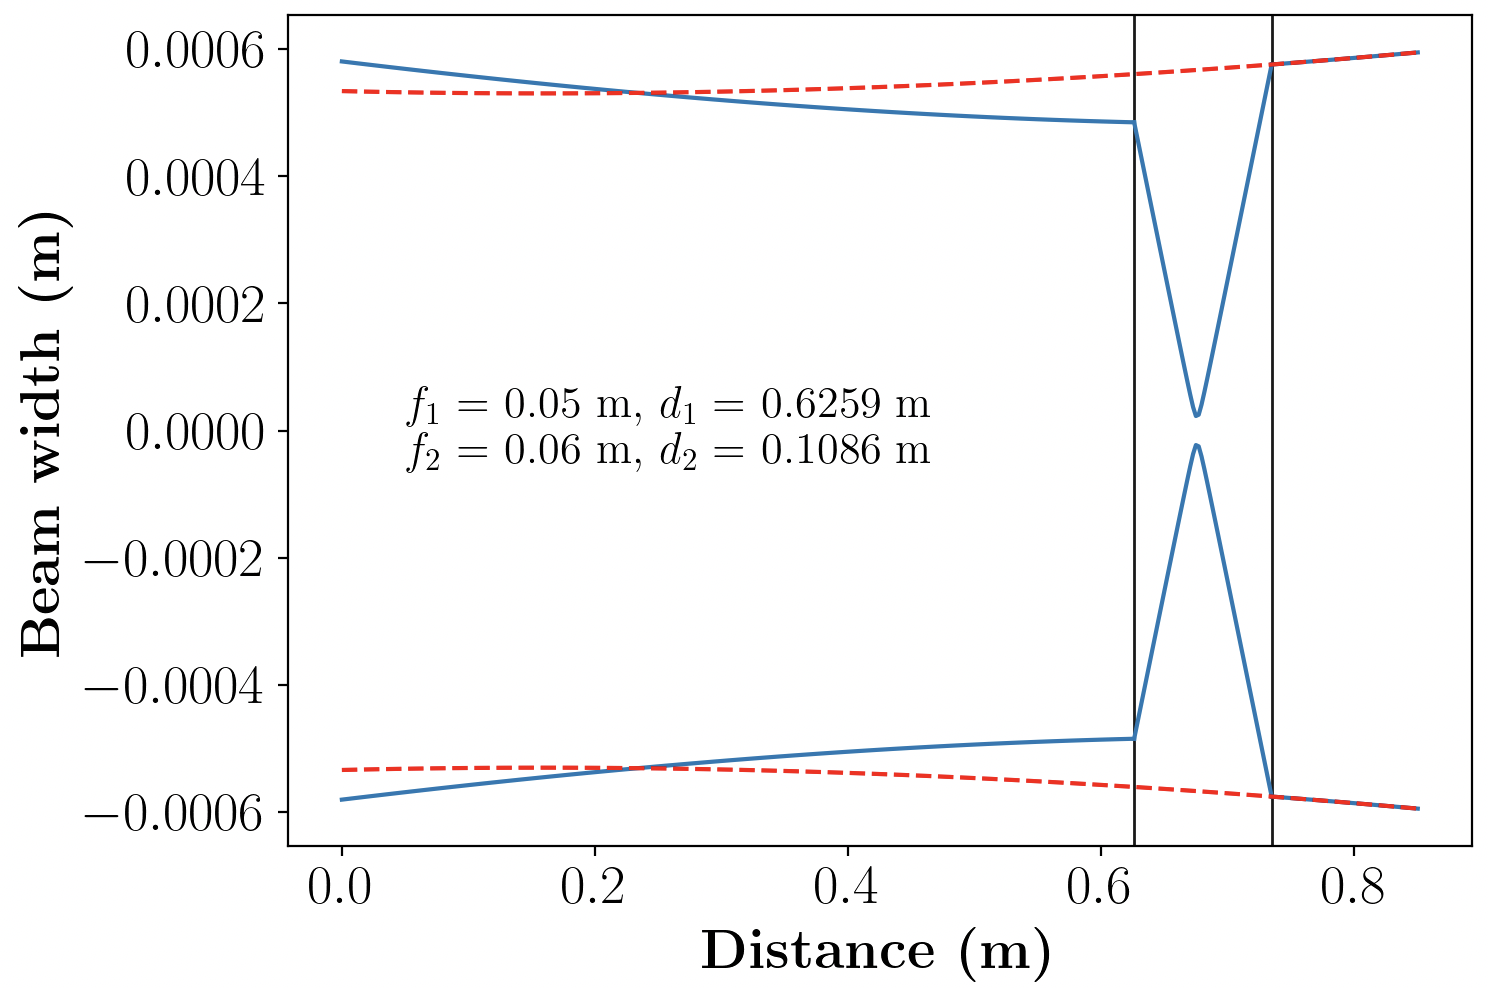
\includegraphics[width=0.9\linewidth]{Figures/OptimalTelescope.png}
    \caption{Beam propagation through the optimised telescope configuration for a laser used in a Mach–Zehnder interferometer in a separate setup. The blue curve shows the calculated Gaussian beam profile after passing through the selected lens pair, while the red dashed curve represents the target fibre-collimated beam profile. The lenses have focal lengths $f_1 = 0.05$~m and $f_2 = 0.06$~m, placed at distances $d_1 = 0.6259$~m and $d_2 = 0.1086$~m from the laser head respectively.}
    \label{fig:optimised-telescope}
\end{figure}


\subsection{Defect Imaging Techniques}

Throughout this project, various search methods were employed to identify high-quality hBN defects. A suitable defect was defined as one that was spatially isolated from other bright emitters, exhibited a high signal-to-noise ratio, and demonstrated temporal stability under continuous excitation.

\subsubsection{APD Scanning Method and Wide Spot Excitation}

The first method used to search for emitters involved scanning a 10~$\mu$m~$\times$~10~$\mu$m area of the sample in a square grid, with the APD collecting counts at 250~nm step intervals. At each point, photon counts were recorded over a 100~ms integration time. This produced a spatial photoluminescence map of the region, from which individual emitters could be readily identified, as shown in Fig.~\ref{fig:apd-scan}.

\begin{figure}[h!]
    \centering

    \begin{subfigure}[b]{0.48\textwidth}
        \centering
        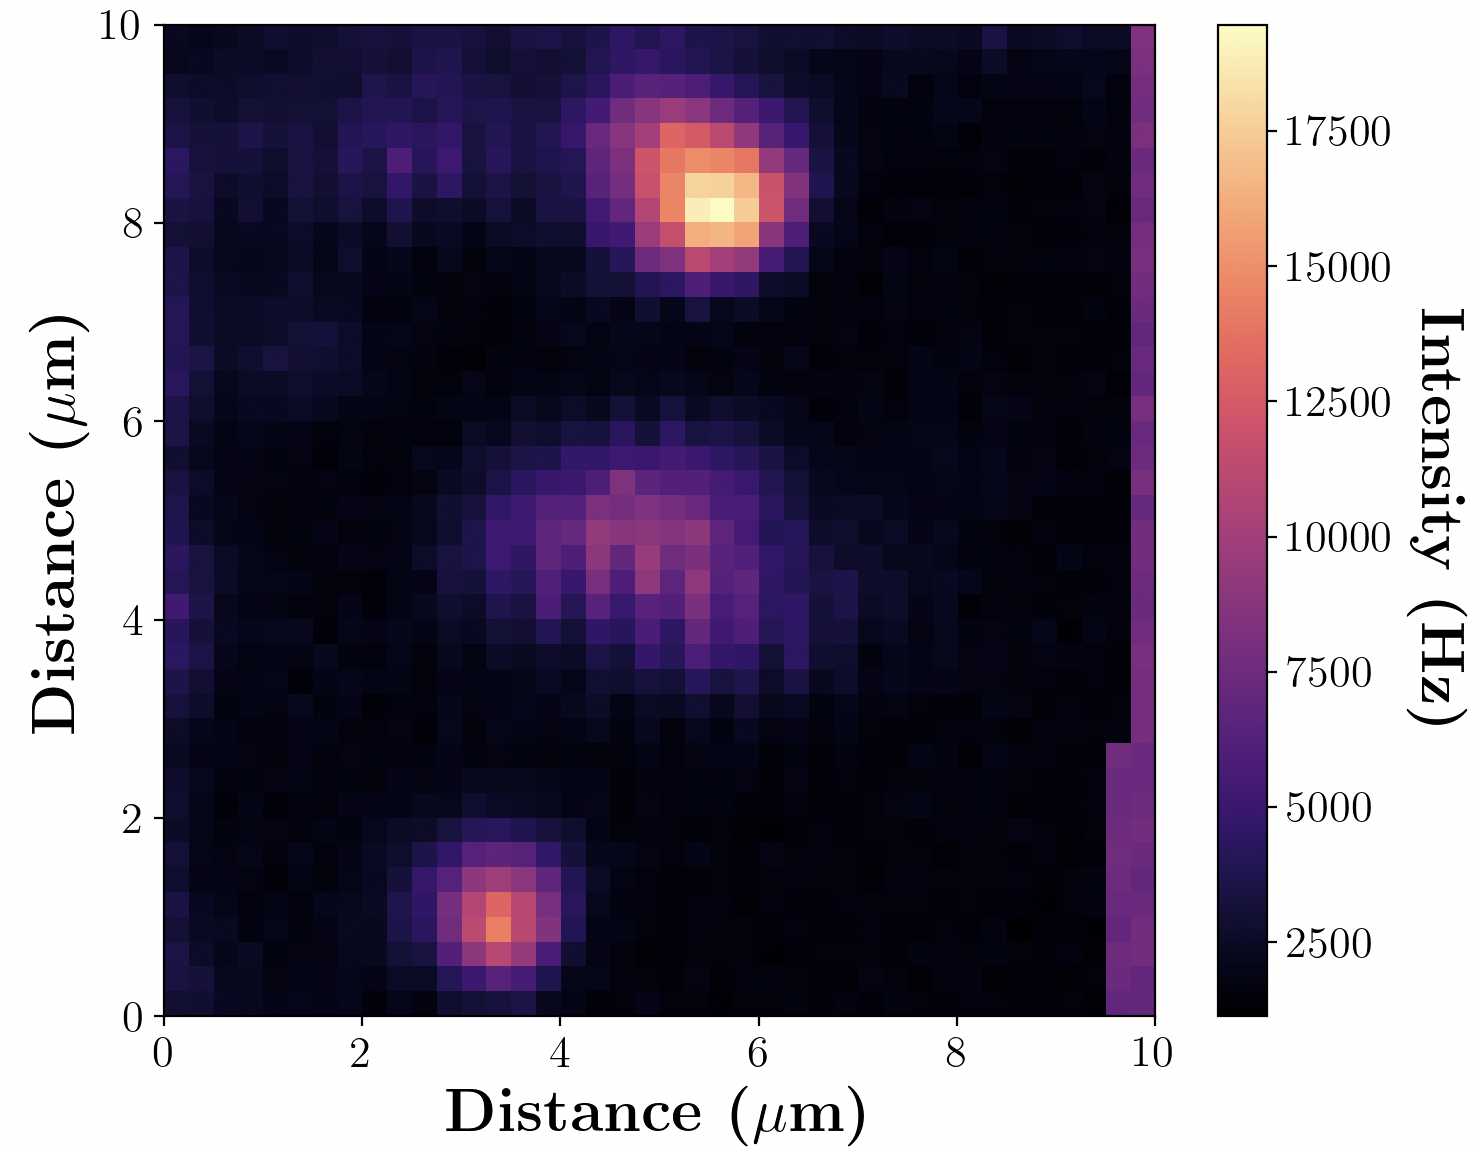
\includegraphics[width=\linewidth]{Figures/APDScan.png}
        \caption{Spatial photoluminescence map of a 10~$\mu$m~$\times$~10~$\mu$m region acquired via wide spot excitation and APD scanning. The scan was performed in 250~nm steps with 100~ms integration time at each position. Brighter regions correspond to higher photon counts, indicating potential emitter locations.}
        \label{fig:apd-scan}
    \end{subfigure}
    \hfill
    \begin{subfigure}[b]{0.48\textwidth}
        \centering
        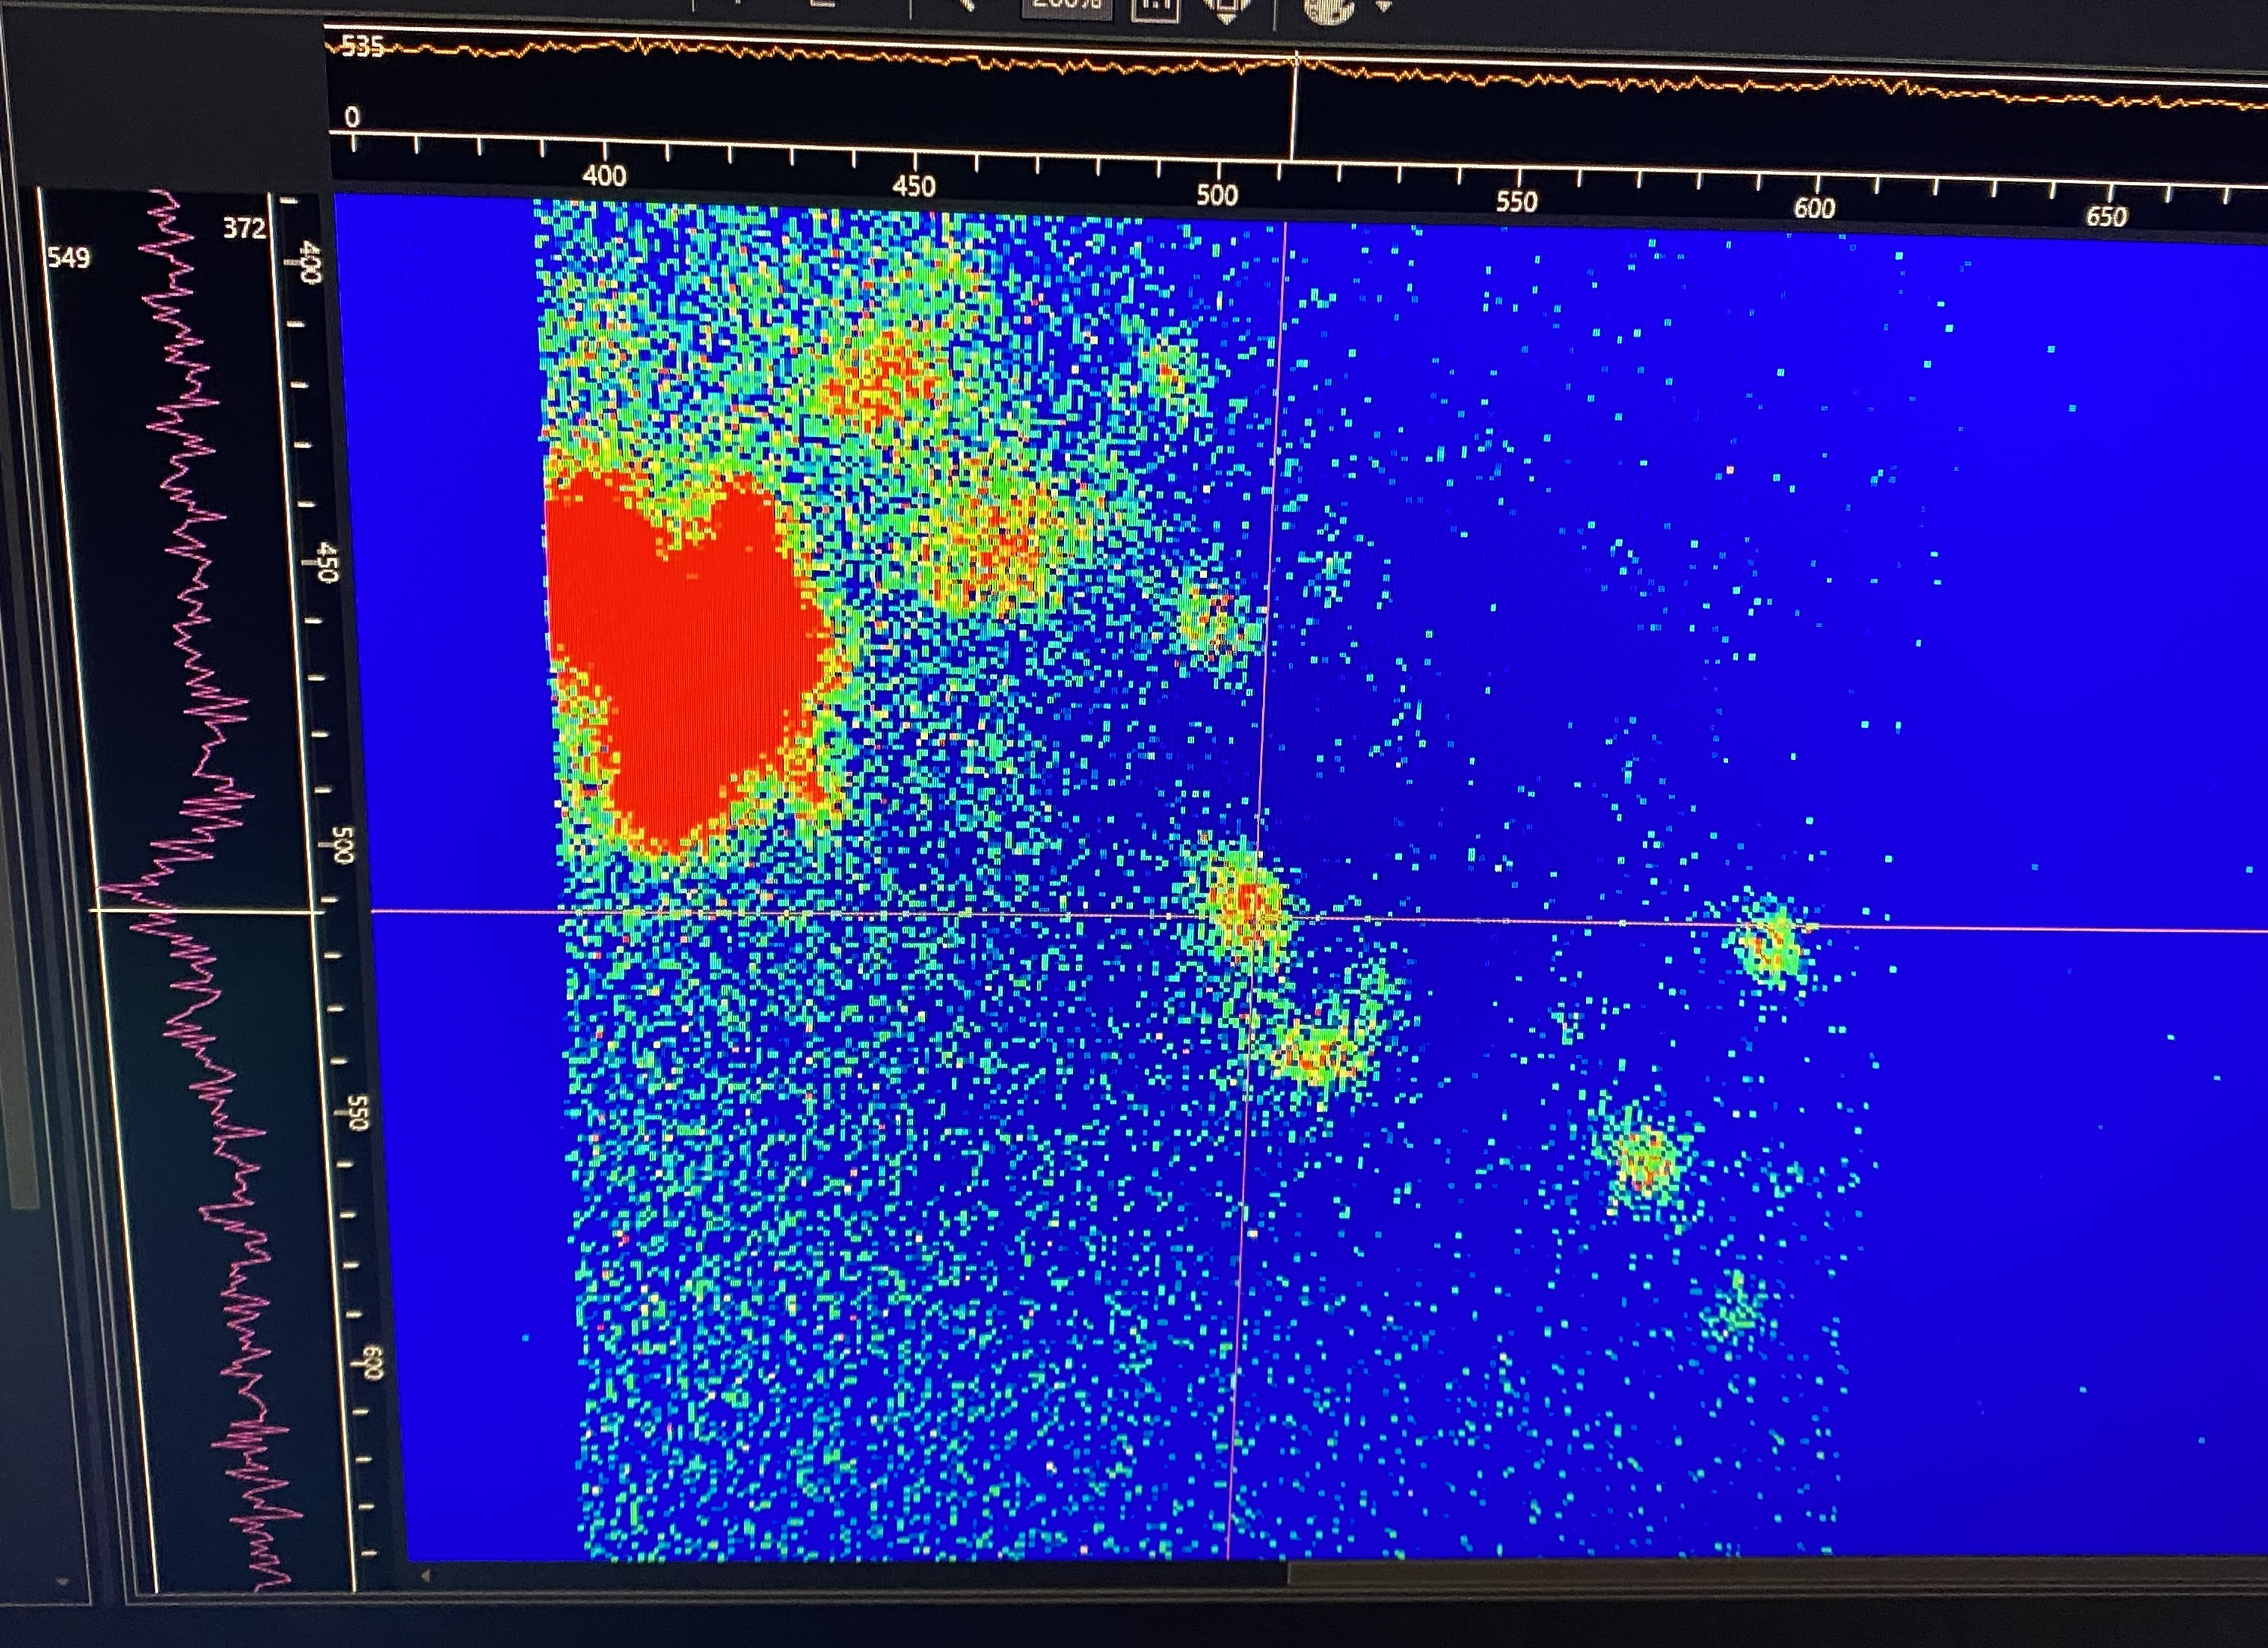
\includegraphics[width=\linewidth]{Figures/WideFieldExcitation.jpg}
        \caption{Wide-spot excitation method for rapid emitter identification. A lens before the objective broadens the excitation beam on the sample, enabling larger-area illumination. Emission is directed to the spectrometer, where bright regions are quickly located by visualising the full sensor output in LightField.}
        \label{fig:wide-field}
    \end{subfigure}

    \caption{(a) APD scanning map and (b) wide-field excitation method for emitter localisation.}
    \label{fig:comparison-methods}
\end{figure}

While effective at locating individual defects, this method is relatively inefficient due to the long acquisition time—approximately three minutes per scan—combined with the limited area covered. This makes it impractical for scanning large areas of the sample. 

Another method used to locate potential emitters was wide-spot imaging. This was achieved by placing a \textcolor{red}{X~mm} focal length lens before the objective, such that the excitation laser was focused at the back focal plane of the objective. As a result, the laser spot on the sample surface became significantly larger, allowing for excitation over a broader area. The collected emission was directed to the spectrometer, and the entire sensor was visualised in the LightField software. This allowed bright emission sites to be identified instantly and enabled rapid scanning across the sample, considerably faster than the previously discussed APD scanning method.

While both the wide-spot and APD scanning methods were effective at locating bright emission sites, a major drawback was that brightness alone did not guarantee quality defects. In practice, most of the initially identified spots exhibited noisy or spectrally impure signals upon closer inspection, rendering them unsuitable for further studies.

\subsubsection{Random Search and Spatial Referencing System}

The most efficient search method for locating bright, isolated defects was found to be a random search approach. In this method, a randomly chosen hBN flake, identified on the CMOS camera, was excited using the 450~nm laser, and the emission was directed to the spectrometer for real-time spectrum visualisation. A manual random walk was then performed using the Attocube nanopositioners, whereby the sample position was adjusted until either a suitable emitter was found or the search was abandoned and a new flake was selected. An example of hBN flakes visible on the CMOS during this process is shown in Fig.~\ref{fig:CMOS-vis}.

\begin{figure}[h]
    \centering
    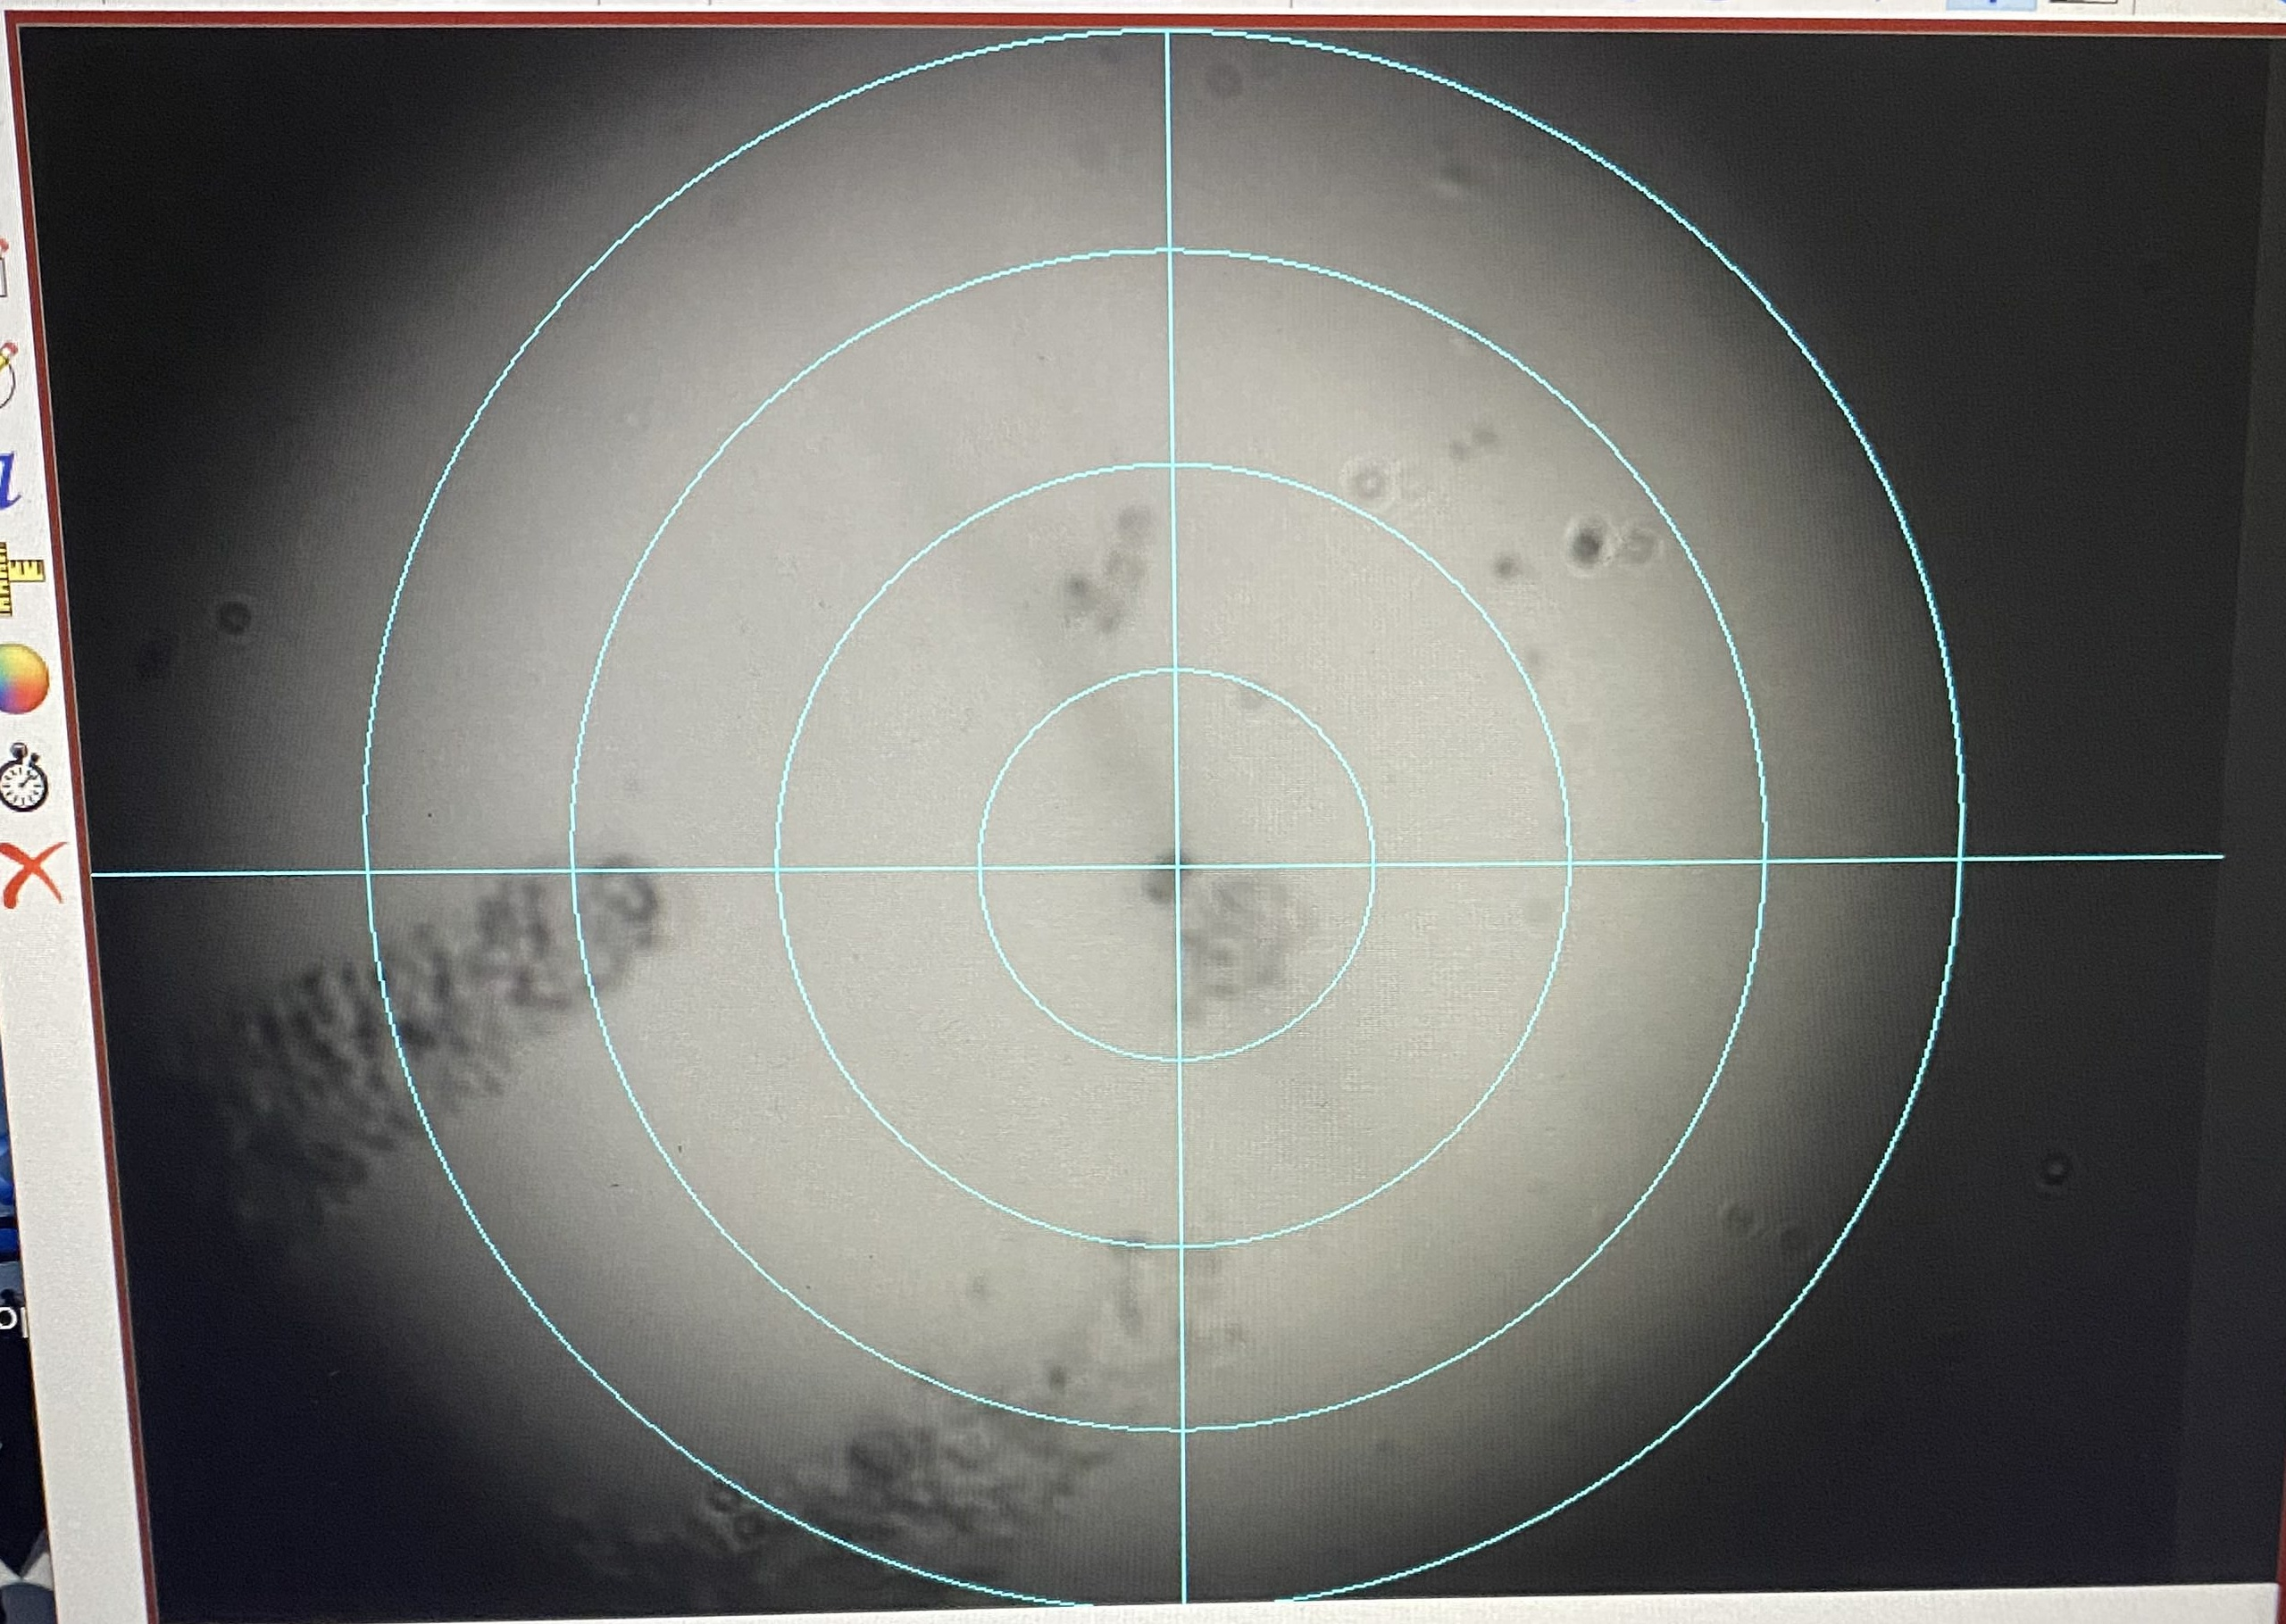
\includegraphics[width=0.75\linewidth]{Figures/CMOS-vis.jpg}
    \caption{CMOS image showing multiple hBN flakes used in the random search method for identifying optically active defects.}
    \label{fig:CMOS-vis}
\end{figure}

This method proved to be the most efficient and reliable for locating promising defects. To ensure that identified emitters could be reliably revisited, a spatial referencing system was developed. Two well-defined points on the hBN flake were selected to form a reference basis, and their coordinates were recorded using the closed-loop Attocube nanopositioners. Since the sample position could shift due to removal or mechanical drift, the reference points were re-measured at the start of each session. When a new emitter was found, its coordinates were transformed into the original reference frame using a custom program. An application built using \texttt{tkinter} was developed to automate this process and store all recorded emitter positions in a database.


\subsection{hBN Measurements}

\subsubsection{Lifetime and Saturation Curve}

Once an emitter with a suitable spectrum is identified, the first measurements performed are typically a saturation curve and lifetime measurement.

A saturation curve characterises how the emission intensity varies with excitation power and can be measured using either pulsed or CW excitation. The measurement is performed with an isolated ZPL, achieved by manually tuning the reconfigurable bandpass filters, and the collection path is directed to the HBT setup. A custom program was developed to automate the measurement by incrementally increasing the excitation power in 5\% steps, from 0\% to 100\%. At each step, the power is measured using a powermeter, and the total photon counts from both APDs in the HBT setup are recorded over a 100~ms integration time. The power at the powermeter is converted to the power at the source by multiplying by 17/83. The process is repeated five times for each power level, and the mean and standard deviation of the measured intensities are taken as the value and uncertainty of the intensity $I(P)$ at a given excitation power $P$.

The resulting data is fitted using the standard saturation model:

\begin{equation}
    I(P) = \frac{P I_{\infty}}{P + P_{\text{sat}}},
    \label{eqn:p-sat}
\end{equation}

where $I_{\infty}$ is the theoretical maximum emission intensity at infinite excitation power, and $P_{\text{sat}}$ is the saturation power, defined as the excitation power at which the emitter reaches half of its maximum intensity. As discussed in Section~\ref{sec:coherence-time}, identifying the saturation power of an emitter prior to further measurements is essential, as excitation powers exceeding this threshold can lead to a significant increase in inhomogeneous broadening.

The lifetime of an emitter is measured using pulsed laser excitation, usually operated at a repetition rate of 40~MHz. A trigger signal from the laser controller (an electrical pulse generated with each pulse emission) is connected to the start channel of the QuTag TCSPC module. MPD APD1 is used for detection and is connected to the initial fibre coupling, before the fibre beam splitter, to maximise the collection of single-photon events. The output signal from the APD is connected to one of the input channels of the QuTag module, using the appropriate trigger level as specified in Table~\ref{tab:apd_characterisatoin}. Photon arrival times are recorded using the software \textit{Daisy}, with a typical acquisition window of 25~ns and a bin size of 25~ps.

The lifetime data provides an initial indication of whether the emitter behaves as a true single-photon source. For an ideal two-level system, the decay curve will exhibit a single exponential shape. In contrast, systems with more than two energy levels, or spatially overlapping defects, often produce multi-exponential decays due to the presence of additional recombination pathways. If the measured decay is consistent with a two-level system, the data is fitted with a single-exponential function:

\begin{equation}
    I(t) = A e^{-\frac{t}{T_1}},
    \label{eqn:lifetime}
\end{equation}

where $I(t)$ is the photon count rate at time $t$ after the trigger signal, $A$ is the initial amplitude (the maximum number of detected photons), and $T_1$ is the lifetime of the emitter, representing the characteristic time scale of spontaneous emission.


\subsubsection{Hanbury Brown and Twiss and $\mathbf{g^{(2)}(0)}$}

The Hanbury Brown and Twiss (HBT) setup is used to measure the second-order correlation function, $g^{(2)}(\tau)$, by recording the arrival times of photons detected by two Thorlabs APDs. Data acquisition is carried out using the \textit{Tarec} (quTag Record \& Merge Tool) software, which logs a timestamp for every detection event. The resulting raw time-tagged data is then analysed using the \textit{Extensible Time-tag Analyzer} (\textit{ETA}), which allows custom histogram generation with flexible bin size and number for varied $g^{(2)}(\tau)$ analysis across both short- and long-timescales.

The HBT setup can be operated under both CW and pulsed excitation schemes. Under CW excitation, the correlation histogram is typically fitted using either a single- or bi-exponential decay function, depending on the underlying emitter dynamics. The single-exponential form is given by:

\begin{equation}
    g^{(2)}(\tau) = A + B e^{-\left| \frac{\tau}{t_0} \right|},
    \label{eqn:single-decay-g2}
\end{equation}

and the bi-exponential form is:

\begin{equation}
    g^{(2)}(\tau) = A + B e^{-\left| \frac{\tau}{t_0} \right|} + C e^{-\left| \frac{\tau}{t_1} \right|},
    \label{eqn:bi-decay-g2}
\end{equation}

\textcolor{red}{blinking - a phenomelological 3rd non-rad decay state}

where $A$ is the baseline offset, $B$ and $C$ are the amplitudes of the respective decay components, and $t_0$ and $t_1$ are the associated decay time constants. For an ideal two-level emitter, the single-exponential model is sufficient. However, in hBN-based single-photon emitters, competing recombination pathways can result in more complex population dynamics. In such cases, a bi-exponential model is required to accurately fit the $g^{(2)}(\tau)$ curve and capture these additional relaxation channels.

The zero-delay value, $g^{(2)}(0)$, is obtained by normalising the coincidence counts at $\tau = 0$ to the baseline at large time delays, i.e. $g^{(2)}(0) = g^{(2)}(0)/g^{(2)}(\infty)$. For the bi-exponential model, this is calculated as $(A + B + C)/A$, and for the single-exponential model, it simplifies to $(A + B)/A$.

In the case of pulsed excitation, the $g^{(2)}(\tau)$ histogram consists of a series of peaks spaced by the repetition period of the laser. To extract $g^{(2)}(0)$, the area under the peak centred at $\tau = 0$ is divided by the average area of peaks at long time delays. It is important to include sufficiently long delay windows in the measurement, as photon bunching effects can result in elevated peaks near zero delay that would otherwise distort the $g^{(2)}(0)$ value.

\subsubsection{Michelson Interferometer and $T_2^*$}

The Michelson interferometer (see Fig.~\ref{fig:setup}) is used to measure the degree of first-order coherence of a single-photon wavepacket by measuring its ability to interfere with itself. One of the mirrors is mounted on a piezoelectric actuator for fine control of the optical path length, while the entire assembly is mounted on a motorised translation stage for coarse adjustment. The piezo actuator has a maximum displacement of 20~$\mu$m, corresponding to a finely tunable optical delay of approximately 67~fs. The translation stage provides up to 5~mm of travel, enabling delay tuning over a broader range of tens of picoseconds (approximately --10~ps to 7~ps).

When the two interferometer arms are equal in length ($\tau = 0$), the wavepacket is expected to interfere constructively with itself, producing a maximum intensity at the output. As the delay $\tau$ is varied, an interference pattern emerges. For example, a small shift of $\tau = \lambda / (2c)$, where $\lambda$ is the single-photon wavelength and $c$ is the speed of light, at which point destructive interference is expected and a minimum in intensity should be observed. By scanning over fine time delays, typically on the order of a few femtoseconds, an interference fringe pattern is obtained. The visibility of this interference pattern is defined as:

\begin{equation}
    V = \frac{I_\text{max} - I_\text{min}}{I_\text{max} + I_\text{min}},
\end{equation}

where $I_\text{max}$ and $I_\text{min}$ are the maximum and minimum intensities of the interference fringes. At zero time delay, perfect phase coherence yields a theoretical visibility $V = 1$. However, if one arm of the interferometer is displaced, by say a several hundred femtoseconds, the visibility $V$ decreases due to pure dephasing of the photon wavepacket. This behaviour can be understood by considering how a pure single-photon state evolves as it passes through a Michelson interferometer.

A pure (perfectly indistinguishable) single-photon can be described as~\textcolor{red}{[reference]}:

\begin{equation}
\begin{aligned}
    \ket{1} & = -i\int_{-\infty}^{\infty} dt\, \sqrt{\gamma} e^{-\frac{t}{2}(\gamma+2i\omega_0)} \Theta(t) \hat{a}^{\dagger}(t) \ket{0}, \\
    & = \int_{-\infty}^{\infty} dt f(t) \hat{a}^{\dagger}(t) \ket{0},
    \label{eqn:wavepacket}
\end{aligned}
\end{equation}

where $\gamma$ is the spontaneous decay rate of the emitter, $\omega_0$ is the central frequency of the single-photon wavepacket, $\Theta(t)$ is the Heaviside step function (ensuring only positive times are considered), and $\hat{a}^{\dagger}(t)$ is the time-dependent photon creation operator in the Fock basis. 

In the presence of pure dephasing at rate $\gamma^*$, the input photon density matrix is modified as:


\begin{equation}
    \rho_{in} = \int_{-\infty}^{\infty}\int_{-\infty}^{\infty}dt \ dt' f(t)f^*(t') \hat{a}^{\dagger}(t) \ket{0} \bra{0} \hat{a}(t) e^{-\gamma^*|t-t'|}.
\end{equation}

To model the evolution of this state through a Michelson interferometer, it is convenient to consider the topologically equivalent case of a Mach–Zehnder interferometer with one delayed arm, as illustrated in Fig.~\ref{fig:MachZhenderMichelson}.


\begin{figure}[h]
    \centering
    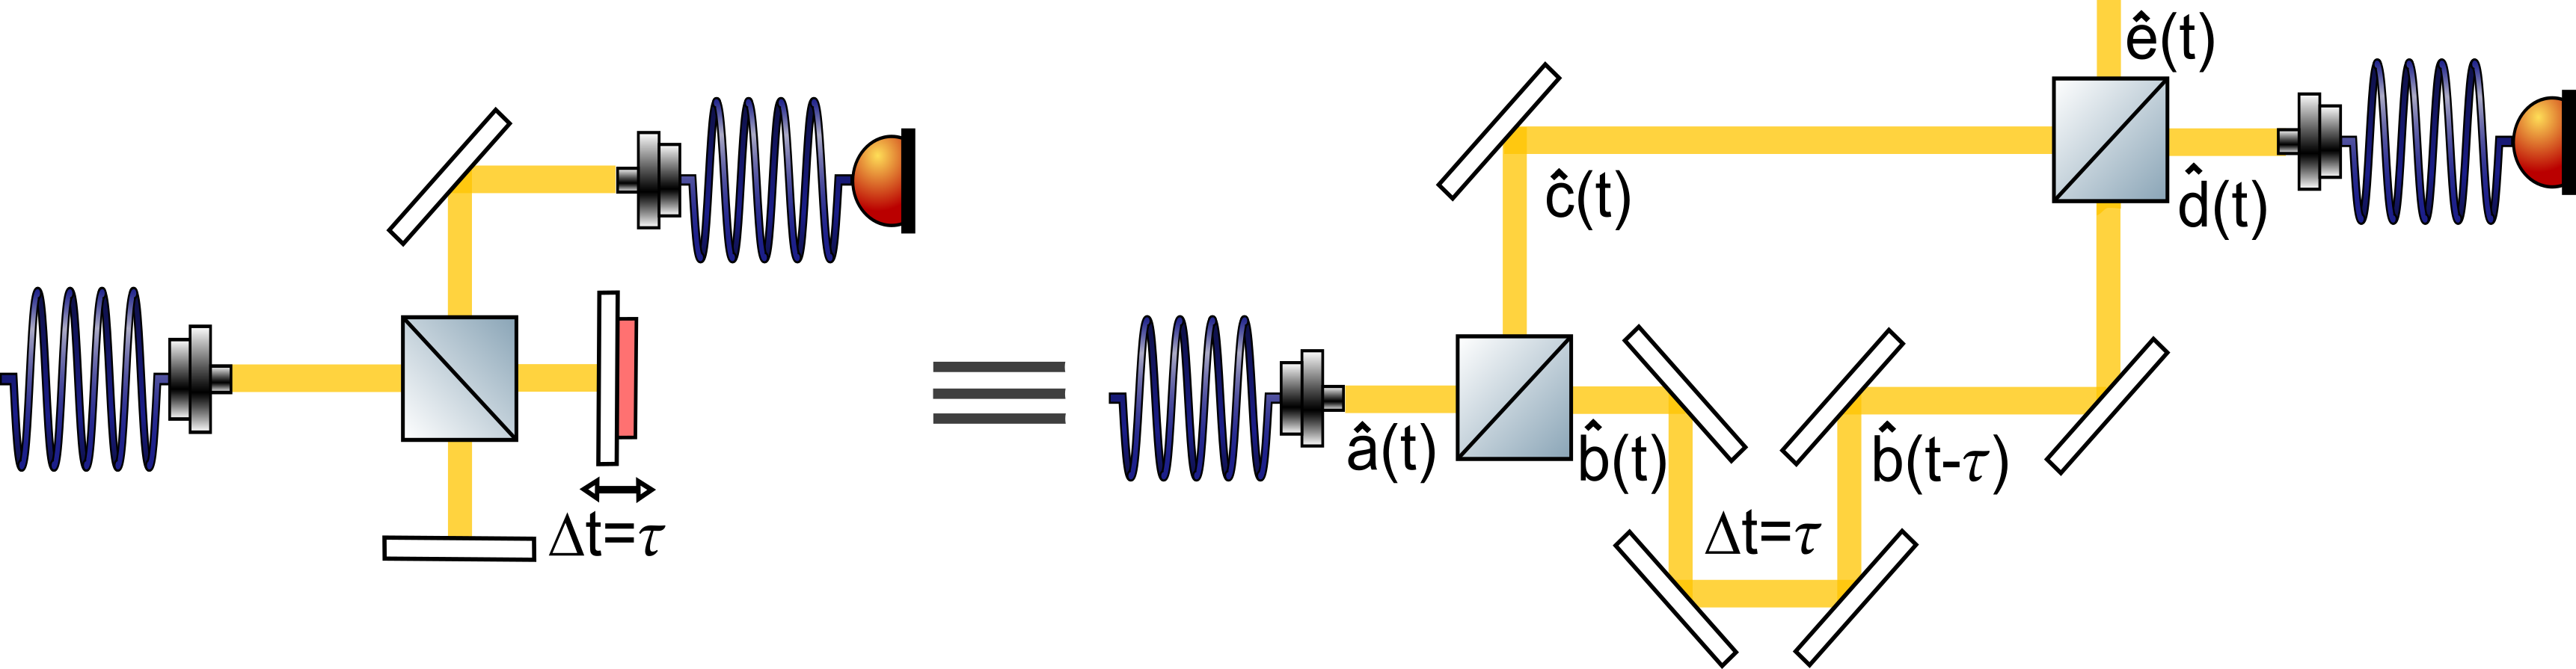
\includegraphics[width=0.8\linewidth]{Figures/MachZhenderMichelson.png}
    \caption{Equivilance of a Mach Zhender interferometer with time delay $\tau$ and a Michelson interferometer. They are both topoligically equivilent, and an analysis of the Mach-Zhender is performed for ease.}
    \label{fig:MachZhenderMichelson}
\end{figure}

Using standard beam splitter conventions~\textcolor{red}{[insert reference]}, the field operators evolve as:


\begin{align}
    \hat{a}(t) & \rightarrow \frac{1}{\sqrt{2}}\left(\hat{b}(t) + \hat{c}(t) \right) \label{eqn:MZ1}\\
    \hat{b}(t) & \rightarrow \hat{b}(t-\tau) \label{eqn:MZ2}\\
    \hat{b}(t-\tau) & \rightarrow \frac{1}{\sqrt{2}}\left(\hat{e}(t-\tau) + \hat{d}(t-\tau) \right) \label{eqn:MZ3}\\
    \hat{c}(t) & \rightarrow \frac{1}{\sqrt2} \left( \hat{e}(t)-\hat{d}(t)\right) \label{eqn:MZ4}
\end{align}

Applying these transformations, the output density matrix becomes:

\begin{equation}
\begin{aligned}
    \rho_{out} = \int_{-\infty}^{\infty}\int_{-\infty}^{\infty}dt \ dt' f(t)f^*(t') e^{-\gamma^*|t-t'|} \times \\ 
    \left[\hat{d}^{\dagger}(t)+\hat{d}^{\dagger}(t-\tau)-\hat{e}^{\dagger}(t) + \hat{e}^{\dagger}(t-\tau)\right]
    \ket{0} \bra{0} \times \\
    \left[\hat{d}(t)+\hat{d}(t-\tau)-\hat{e}(t) + \hat{e}(t-\tau)\right],
\end{aligned}
\end{equation}

The photon intensity measured at output port $\hat{d}(t)$ is given by:

\begin{equation}
\begin{aligned}
    N_d(t'') 
    &= \langle \hat{d}^{\dagger}(t'') \hat{d}(t'') \rangle 
    = \text{Tr}\left[\hat{\rho}_{out} \, \hat{d}^{\dagger}(t'') \hat{d}(t'')\right] \\
    &= \int_{-\infty}^{\infty} \int_{-\infty}^{\infty} dt \, dt' \, f(t) f e^{-\gamma^*|t - t'|} \\
    &\quad \times \text{Tr} \Big[ 
        \left( \hat{d}^{\dagger}(t) + \hat{d}^{\dagger}(t - \tau) 
              - \hat{e}^{\dagger}(t) + \hat{e}^{\dagger}(t - \tau) \right) 
        \ket{0} \bra{0} \\
    &\hspace{1.7cm}
         \left( \hat{d}(t) + \hat{d}(t - \tau) 
              - \hat{e}(t) + \hat{e}(t - \tau) \right)
        \hat{d}^{\dagger}(t'') \hat{d}(t'') 
    \Big] \\
    &= \int_{-\infty}^{\infty} \int_{-\infty}^{\infty} dt \, dt' \, f(t) f^*(t') e^{-\gamma^*|t - t'|} \\
    &\quad \times \big[ 
        \delta(t - t'') \delta(t' - t'') 
        + \delta(t - \tau - t'') \delta(t' - t'') \\
    &\qquad 
        + \delta(t - t'') \delta(t' - \tau - t'') 
        + \delta(t - \tau - t'') \delta(t' - \tau - t'') 
    \big] \\
    &= |f(t'')|^2 + |f(\tau+t'')|^2 + 2\text{Re}\left[f(t'')f^*(\tau+t'')e^{-\gamma^* \tau } \right]\\
\end{aligned}
\end{equation}

For the wavepacket described in equation~\ref{eqn:wavepacket}, this results in:

\begin{equation}
    N_d(t'') = \frac{\gamma}{4} e^{-\gamma t''} \left[\Theta(t'') + \Theta(t'' - \tau) e^{-\gamma \tau} + 2 \cos(\omega_0 \tau)\, e^{-\gamma t'' - \gamma^* \tau} \Theta(t'') \Theta(t'' - \tau) \right].
\end{equation}

Integrating over all time gives the total photon number at detector $\hat{d}$:

\begin{equation}
\begin{aligned}
    N_d &= \int_{-\infty}^{\infty} dt''\, N_d(t'') \\
        &= \frac{1}{2} \left(1 + e^{-\frac{1}{2}(\gamma + 2\gamma^*) \tau} \cos(\omega_0 \tau) \right) \\
        &= \frac{1}{2} \left(1 + e^{-\frac{1}{2} \Gamma \tau} \cos(\omega_0 \tau) \right),
\end{aligned}
\end{equation}

This result shows that the measured intensity at the output oscillates with frequency $\omega_0$ and decays exponentially with delay $\tau$ due to the combined effect of spontaneous emission and pure dephasing. The envelope of this decay gives direct access to the emitter’s coherence properties and allows extraction of the dephasing rate $\gamma^*$.

To perform the measurement, the piezo actuator is driven with a triangular waveform between 0.5~V and 9.5~V at a repetition rate of 10~Hz, generated by a \textcolor{red}{[INSERT waveform generator model]}. A synchronised CMOS trigger output from the same generator is used to start the QuTag TCSPC system. The interference signal at the output of the interferometer is coupled into a single-mode fibre and detected using a Thorlabs APD. Photon arrival times are recorded relative to the trigger signal, with the delay $\tau$ assumed to vary linearly over the piezo scan range. To access longer delays, the motorised translation stage is repositioned to introduce a new optical path difference, and the measurement is repeated.


\subsection{Cavity Design}

To enhance the rate of spontaneous emission from hBN defects, an open Fabry–Pérot cavity was employed to couple the emitter’s radiation into a well-defined optical mode. The cavity consists of a bottom planar distributed Bragg reflector (DBR) mirror, onto which the hBN flake is dropcast, and a top DBR mirror incorporating a mesa structure patterned with two 3$\times$5 arrays of concave mirrors. Each array consists of concave mirrors that are identical in both diameter and depth within the array, but the two arrays differ from each other in mirror depth while having the same diameter. The DBR mirrors are formed from alternating layers of SiO$_2$ and TiO$_2$, which reflect light via constructive interference due to the periodic variation in refractive index.

The mesa structure has dimensions of 0.1~mm~$\times$~0.1~mm~$\times$~0.1~mm and elevates the concave mirrors, allowing the top and bottom mirrors to be brought into close proximity without the risk of physical contact at their edges. This configuration is essential for minimising the cavity mode volume, as the Purcell factor is inversely proportional to the effective cavity volume.

\begin{figure}[h]
    \centering
    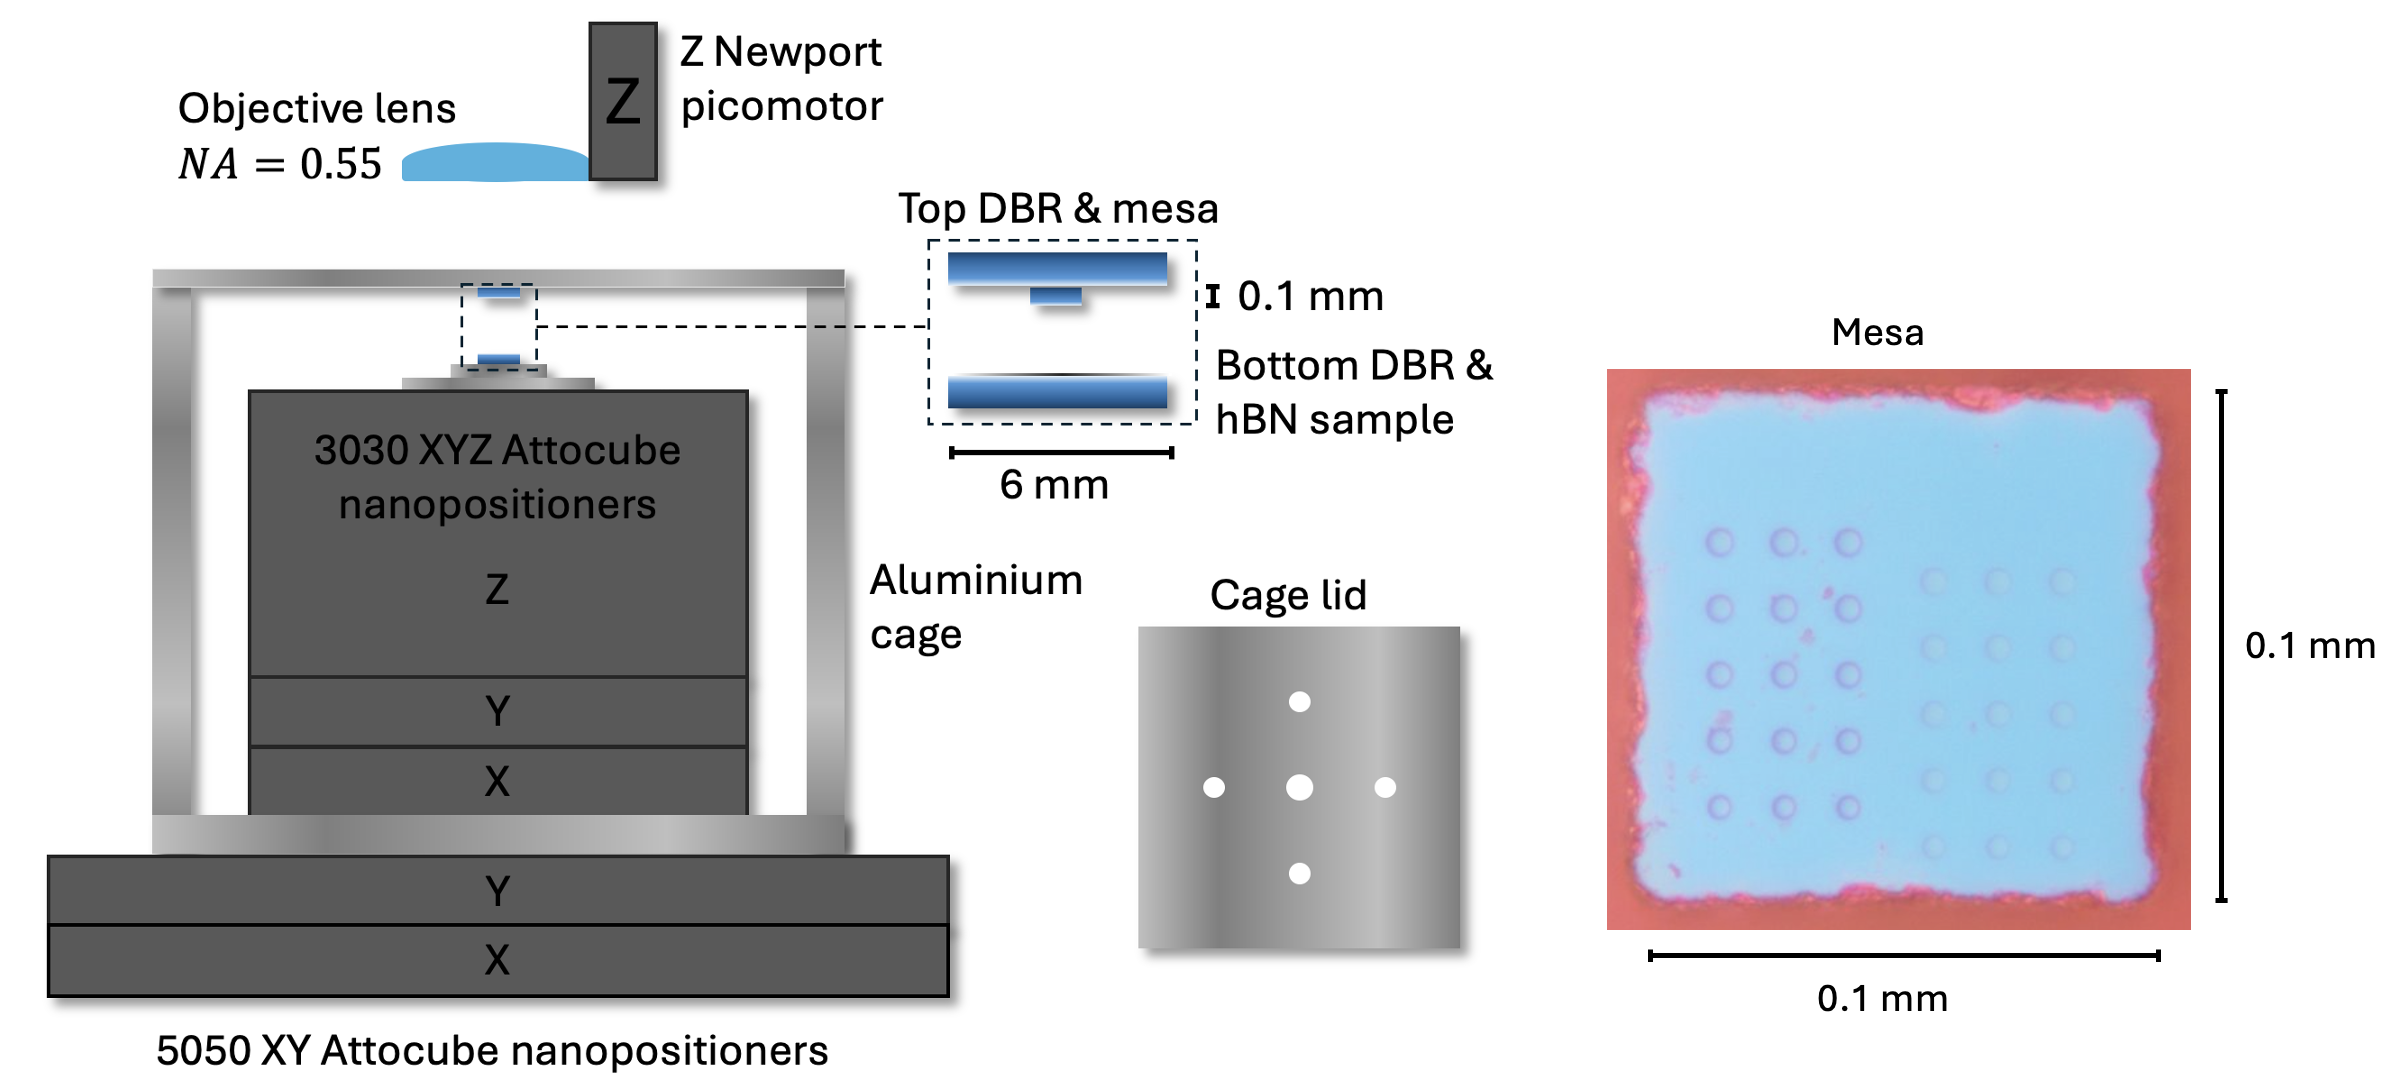
\includegraphics[width=0.9\linewidth]{Figures/CavityDesign1.png}
    \caption{Schematic of the open-access Fabry–Pérot cavity design. The system includes a planar bottom DBR mirror with a dropcast hBN sample, and a top DBR mirror incorporating a mesa containing two 3$\times$5 arrays of concave mirrors with varying depths. A lid with multiple apertures enables optical access and imaging via the CMOS camera. Motorised nanopositioners provide full XYZ control of both the cavity and the sample.}
    \label{fig:cavity-design1}
\end{figure}

The cavity is controlled using two independent sets of Attocube nanopositioners. A set of external 5050 XY closed-loop nanopositioners controls the position of the aluminium cage as a whole, while an internal set of 3030 XYZ nanopositioners allows precise movement of the sample stage within the cage. This dual-stage system enables a multistep procedure for emitter–cavity alignment:

\begin{enumerate}
    \item Using the 5050 XY nanopositioners, locate a concave mirror through the central hole of the cage lid via the CMOS camera. Record the closed-loop position.
    \item Move the 3030 XYZ nanopositioners to shift the sample underneath one of the side apertures of the cage lid. Simultaneously compensate with the 5050 stages to keep the sample visible in the CMOS.
    \item Search for an hBN defect using the 3030 nanopositioners.
    \item Once a suitable emitter is identified, reverse the motion from step 2 to reposition the emitter beneath the previously selected concave mirror, verifying alignment using the CMOS camera.
    \item Excite the emitter and begin closing the cavity by moving the 3030 Z nanopositioner upwards.
\end{enumerate}

A program was developed to automate the procedure described above. High precision, on the order of a few nanometres, is required, as the sample is not visible in the CMOS beneath the top mirror until the mirror separation falls below approximately 10~$\mu$m. As a result, the final stage of the alignment process is effectively performed ``blind" and must be executed with high accuracy to ensure that the selected defect ends up positioned directly below the top concave mirror.

\subsubsection{Top Mirror AFM Measurements}

The DBR mirrors were fabricated at Universität Würzburg, where the atomic force microscopy (AFM) measurements shown in Fig.~\ref{fig:AFM-Measurement} were also performed. The mesa contains two arrays of concave mirrors, each with a diameter of 7~$\mu$m. The mirrors in the shallow array have a depth of around 200~nm, while those in the deep array have a depth of approximately 380~nm.

\begin{figure}[h]
    \centering
    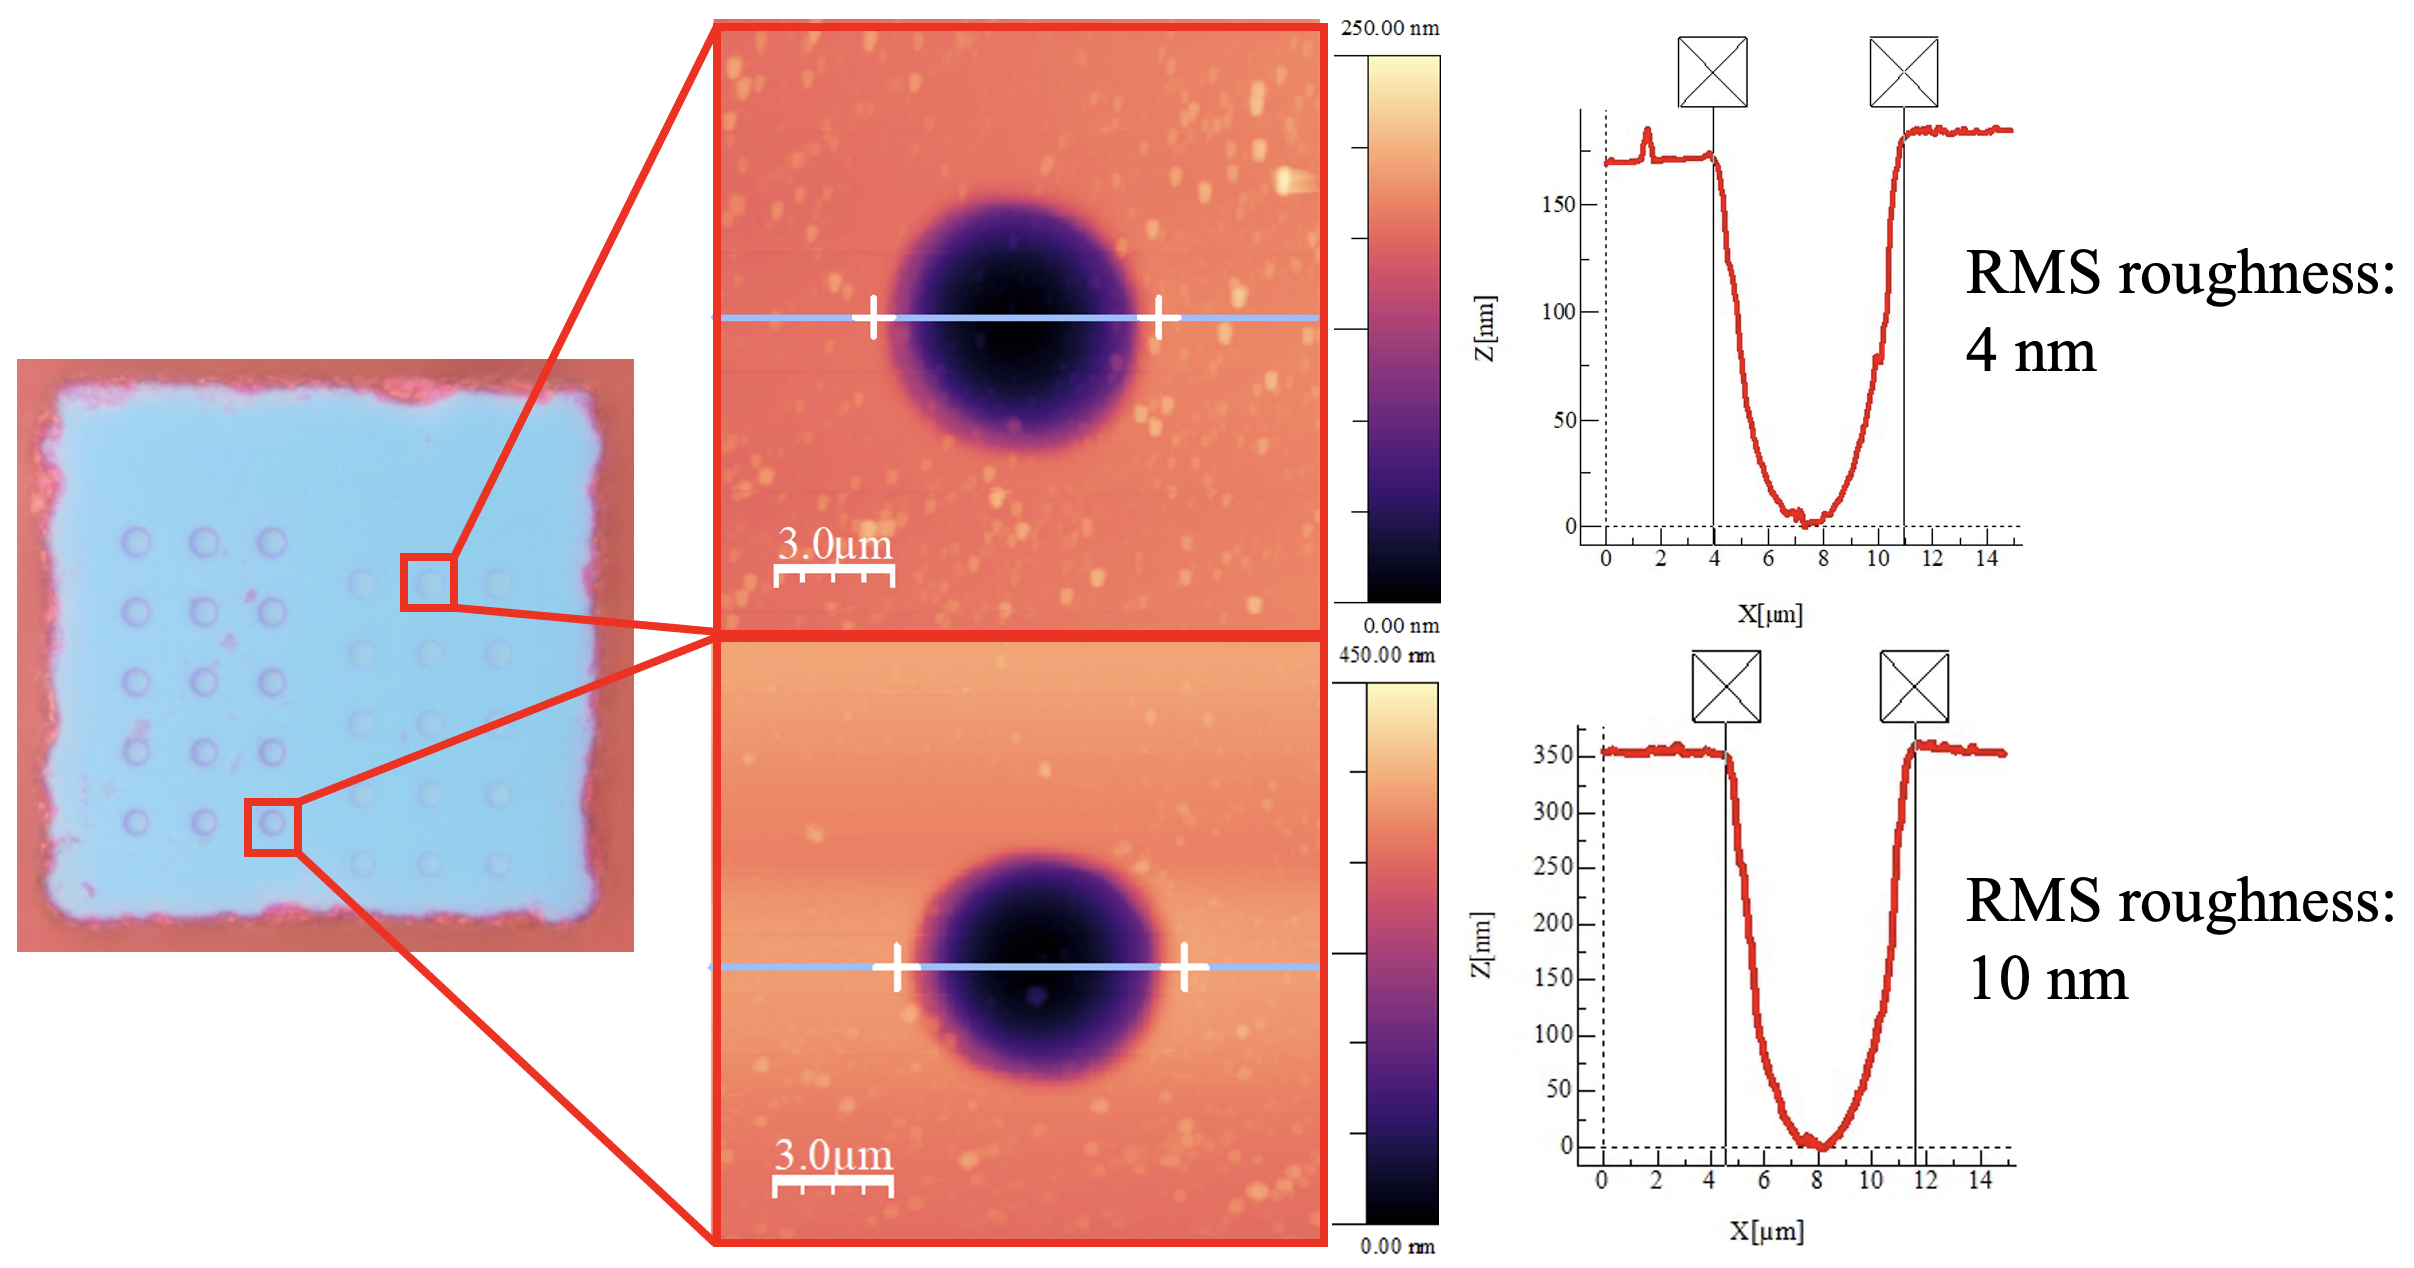
\includegraphics[width=0.9\linewidth]{Figures/MirrorAFM.png}
    \caption{AFM characterisation of concave mirrors fabricated on the mesa structure. The left panel shows the full mesa containing multiple concave mirrors. Zoomed-in AFM scans (centre panels) of mirrors from the shallow and deep arrays reveal the surface profile. The corresponding cross-sectional profiles can be seen in the right panels. The RMS surface roughness was measured to be 4~nm for the shallow mirror and 10~nm for the deeper mirror.}
    \label{fig:AFM-Measurement}
\end{figure}


\subsubsection{DBR Layer Pair Optimisation via Simulation}

The number of DBR layers on the top and bottom mirrors of the cavity must be chosen carefully in order to optimise the Purcell factor of the system. 

The Q-factor of the cavity is defined as the $\lambda_{\text{cav}}/\Gamma$, where $\lambda_{\text{cav}}$ is the central wavelength of the cavity, and $\Gamma$ is the FWHM of the cavities reflectivity curve.




\newpage